\documentclass[1p]{elsarticle_modified}
%\bibliographystyle{elsarticle-num}

%\usepackage[colorlinks]{hyperref}
%\usepackage{abbrmath_seonhwa} %\Abb, \Ascr, \Acal ,\Abf, \Afrak
\usepackage{amsfonts}
\usepackage{amssymb}
\usepackage{amsmath}
\usepackage{amsthm}
\usepackage{scalefnt}
\usepackage{amsbsy}
\usepackage{kotex}
\usepackage{caption}
\usepackage{subfig}
\usepackage{color}
\usepackage{graphicx}
\usepackage{xcolor} %% white, black, red, green, blue, cyan, magenta, yellow
\usepackage{float}
\usepackage{setspace}
\usepackage{hyperref}

\usepackage{tikz}
\usetikzlibrary{arrows}

\usepackage{multirow}
\usepackage{array} % fixed length table
\usepackage{hhline}

%%%%%%%%%%%%%%%%%%%%%
\makeatletter
\renewcommand*\env@matrix[1][\arraystretch]{%
	\edef\arraystretch{#1}%
	\hskip -\arraycolsep
	\let\@ifnextchar\new@ifnextchar
	\array{*\c@MaxMatrixCols c}}
\makeatother %https://tex.stackexchange.com/questions/14071/how-can-i-increase-the-line-spacing-in-a-matrix
%%%%%%%%%%%%%%%

\usepackage[normalem]{ulem}

\newcommand{\msout}[1]{\ifmmode\text{\sout{\ensuremath{#1}}}\else\sout{#1}\fi}
%SOURCE: \msout is \stkout macro in https://tex.stackexchange.com/questions/20609/strikeout-in-math-mode

\newcommand{\cancel}[1]{
	\ifmmode
	{\color{red}\msout{#1}}
	\else
	{\color{red}\sout{#1}}
	\fi
}

\newcommand{\add}[1]{
	{\color{blue}\uwave{#1}}
}

\newcommand{\replace}[2]{
	\ifmmode
	{\color{red}\msout{#1}}{\color{blue}\uwave{#2}}
	\else
	{\color{red}\sout{#1}}{\color{blue}\uwave{#2}}
	\fi
}

\newcommand{\Sol}{\mathcal{S}} %segment
\newcommand{\D}{D} %diagram
\newcommand{\A}{\mathcal{A}} %arc


%%%%%%%%%%%%%%%%%%%%%%%%%%%%%5 test

\def\sl{\operatorname{\textup{SL}}(2,\Cbb)}
\def\psl{\operatorname{\textup{PSL}}(2,\Cbb)}
\def\quan{\mkern 1mu \triangleright \mkern 1mu}

\theoremstyle{definition}
\newtheorem{thm}{Theorem}[section]
\newtheorem{prop}[thm]{Proposition}
\newtheorem{lem}[thm]{Lemma}
\newtheorem{ques}[thm]{Question}
\newtheorem{cor}[thm]{Corollary}
\newtheorem{defn}[thm]{Definition}
\newtheorem{exam}[thm]{Example}
\newtheorem{rmk}[thm]{Remark}
\newtheorem{alg}[thm]{Algorithm}

\newcommand{\I}{\sqrt{-1}}
\begin{document}

%\begin{frontmatter}
%
%\title{Boundary parabolic representations of knots up to 8 crossings}
%
%%% Group authors per affiliation:
%\author{Yunhi Cho} 
%\address{Department of Mathematics, University of Seoul, Seoul, Korea}
%\ead{yhcho@uos.ac.kr}
%
%
%\author{Seonhwa Kim} %\fnref{s_kim}}
%\address{Center for Geometry and Physics, Institute for Basic Science, Pohang, 37673, Korea}
%\ead{ryeona17@ibs.re.kr}
%
%\author{Hyuk Kim}
%\address{Department of Mathematical Sciences, Seoul National University, Seoul 08826, Korea}
%\ead{hyukkim@snu.ac.kr}
%
%\author{Seokbeom Yoon}
%\address{Department of Mathematical Sciences, Seoul National University, Seoul, 08826,  Korea}
%\ead{sbyoon15@snu.ac.kr}
%
%\begin{abstract}
%We find all boundary parabolic representation of knots up to 8 crossings.
%
%\end{abstract}
%\begin{keyword}
%    \MSC[2010] 57M25 
%\end{keyword}
%
%\end{frontmatter}

%\linenumbers
%\tableofcontents
%
\newcommand\colored[1]{\textcolor{white}{\rule[-0.35ex]{0.8em}{1.4ex}}\kern-0.8em\color{red} #1}%
%\newcommand\colored[1]{\textcolor{white}{ #1}\kern-2.17ex	\textcolor{white}{ #1}\kern-1.81ex	\textcolor{white}{ #1}\kern-2.15ex\color{red}#1	}

{\Large $\underline{12a_{0418}~(K12a_{0418})}$}

\setlength{\tabcolsep}{10pt}
\renewcommand{\arraystretch}{1.6}
\vspace{1cm}\begin{tabular}{m{100pt}>{\centering\arraybackslash}m{274pt}}
\multirow{5}{120pt}{
	\centering
	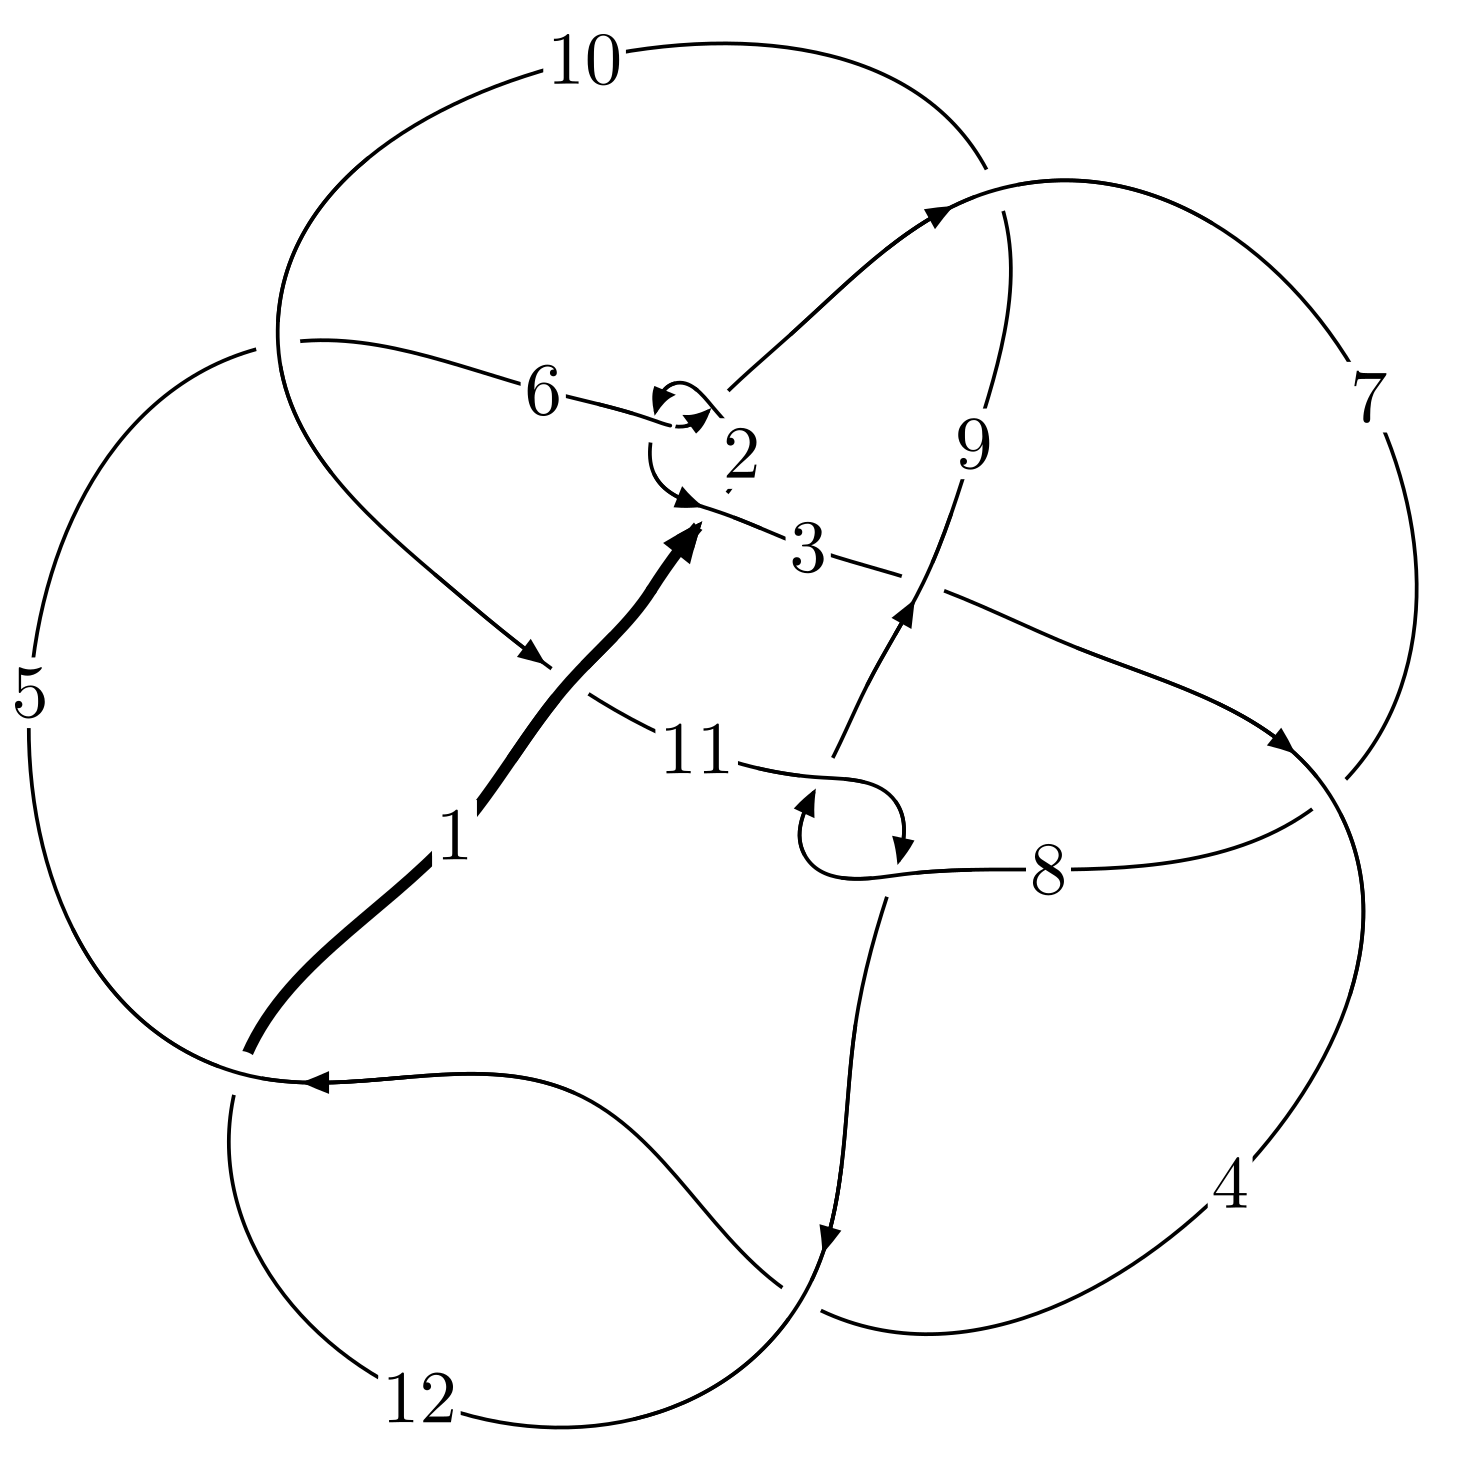
\includegraphics[width=112pt]{../../../GIT/diagram.site/Diagrams/png/1219_12a_0418.png}\\
\ \ \ A knot diagram\footnotemark}&
\allowdisplaybreaks
\textbf{Linearized knot diagam} \\
\cline{2-2}
 &
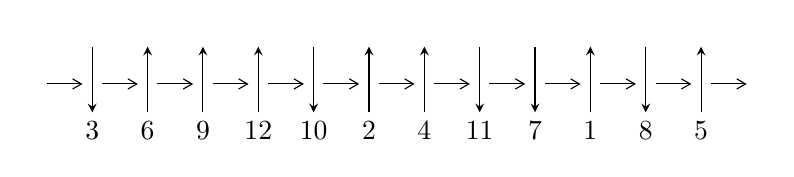
\begin{tikzpicture}[x=20pt, y=17pt]
	% nodes
	\node (C0) at (0, 0) {};
	\node (C1) at (1, 0) {};
	\node (C1U) at (1, +1) {};
	\node (C1D) at (1, -1) {3};

	\node (C2) at (2, 0) {};
	\node (C2U) at (2, +1) {};
	\node (C2D) at (2, -1) {6};

	\node (C3) at (3, 0) {};
	\node (C3U) at (3, +1) {};
	\node (C3D) at (3, -1) {9};

	\node (C4) at (4, 0) {};
	\node (C4U) at (4, +1) {};
	\node (C4D) at (4, -1) {12};

	\node (C5) at (5, 0) {};
	\node (C5U) at (5, +1) {};
	\node (C5D) at (5, -1) {10};

	\node (C6) at (6, 0) {};
	\node (C6U) at (6, +1) {};
	\node (C6D) at (6, -1) {2};

	\node (C7) at (7, 0) {};
	\node (C7U) at (7, +1) {};
	\node (C7D) at (7, -1) {4};

	\node (C8) at (8, 0) {};
	\node (C8U) at (8, +1) {};
	\node (C8D) at (8, -1) {11};

	\node (C9) at (9, 0) {};
	\node (C9U) at (9, +1) {};
	\node (C9D) at (9, -1) {7};

	\node (C10) at (10, 0) {};
	\node (C10U) at (10, +1) {};
	\node (C10D) at (10, -1) {1};

	\node (C11) at (11, 0) {};
	\node (C11U) at (11, +1) {};
	\node (C11D) at (11, -1) {8};

	\node (C12) at (12, 0) {};
	\node (C12U) at (12, +1) {};
	\node (C12D) at (12, -1) {5};
	\node (C13) at (13, 0) {};

	% arrows
	\draw[->,>={angle 60}]
	(C0) edge (C1) (C1) edge (C2) (C2) edge (C3) (C3) edge (C4) (C4) edge (C5) (C5) edge (C6) (C6) edge (C7) (C7) edge (C8) (C8) edge (C9) (C9) edge (C10) (C10) edge (C11) (C11) edge (C12) (C12) edge (C13) ;	\draw[->,>=stealth]
	(C1U) edge (C1D) (C2D) edge (C2U) (C3D) edge (C3U) (C4D) edge (C4U) (C5U) edge (C5D) (C6D) edge (C6U) (C7D) edge (C7U) (C8U) edge (C8D) (C9U) edge (C9D) (C10D) edge (C10U) (C11U) edge (C11D) (C12D) edge (C12U) ;
	\end{tikzpicture} \\
\hhline{~~} \\& 
\textbf{Solving Sequence} \\ \cline{2-2} 
 &
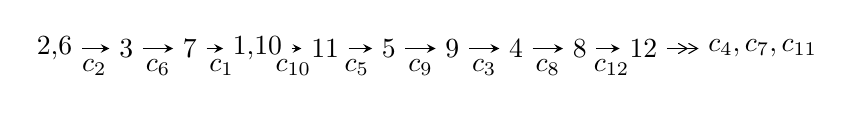
\begin{tikzpicture}[x=23pt, y=7pt]
	% node
	\node (A0) at (-1/8, 0) {2,6};
	\node (A1) at (1, 0) {3};
	\node (A2) at (2, 0) {7};
	\node (A3) at (49/16, 0) {1,10};
	\node (A4) at (33/8, 0) {11};
	\node (A5) at (41/8, 0) {5};
	\node (A6) at (49/8, 0) {9};
	\node (A7) at (57/8, 0) {4};
	\node (A8) at (65/8, 0) {8};
	\node (A9) at (73/8, 0) {12};
	\node (C1) at (1/2, -1) {$c_{2}$};
	\node (C2) at (3/2, -1) {$c_{6}$};
	\node (C3) at (5/2, -1) {$c_{1}$};
	\node (C4) at (29/8, -1) {$c_{10}$};
	\node (C5) at (37/8, -1) {$c_{5}$};
	\node (C6) at (45/8, -1) {$c_{9}$};
	\node (C7) at (53/8, -1) {$c_{3}$};
	\node (C8) at (61/8, -1) {$c_{8}$};
	\node (C9) at (69/8, -1) {$c_{12}$};
	\node (A10) at (11, 0) {$c_{4},c_{7},c_{11}$};

	% edge
	\draw[->,>=stealth]	
	(A0) edge (A1) (A1) edge (A2) (A2) edge (A3) (A3) edge (A4) (A4) edge (A5) (A5) edge (A6) (A6) edge (A7) (A7) edge (A8) (A8) edge (A9) ;
	\draw[->>,>={angle 60}]	
	(A9) edge (A10);
\end{tikzpicture} \\ 

\end{tabular} \\

\footnotetext{
The image of knot diagram is generated by the software ``\textbf{Draw programme}" developed by Andrew Bartholomew(\url{http://www.layer8.co.uk/maths/draw/index.htm\#Running-draw}), where we modified some parts for our purpose(\url{https://github.com/CATsTAILs/LinksPainter}).
}\phantom \\ \newline 
\centering \textbf{Ideals for irreducible components\footnotemark of $X_{\text{par}}$} 
 
\begin{align*}
I^u_{1}&=\langle 
1.94917\times10^{418} u^{163}+1.81536\times10^{418} u^{162}+\cdots+9.84278\times10^{417} b+3.97689\times10^{418},\\
\phantom{I^u_{1}}&\phantom{= \langle  }6.96715\times10^{418} u^{163}+2.22660\times10^{419} u^{162}+\cdots+9.84278\times10^{417} a-9.30364\times10^{417},\\
\phantom{I^u_{1}}&\phantom{= \langle  }u^{164}+3 u^{163}+\cdots+12 u-1\rangle \\
I^u_{2}&=\langle 
-6087254789723 u^{40}+551946361063 u^{39}+\cdots+4003363922926 b-35131970365899,\\
\phantom{I^u_{2}}&\phantom{= \langle  }-25612286566117 u^{40}-31874660592809 u^{39}+\cdots+4003363922926 a-38454939383807,\\
\phantom{I^u_{2}}&\phantom{= \langle  }u^{41}+2 u^{40}+\cdots+8 u+1\rangle \\
\\
\end{align*}
\raggedright * 2 irreducible components of $\dim_{\mathbb{C}}=0$, with total 205 representations.\\
\footnotetext{All coefficients of polynomials are rational numbers. But the coefficients are sometimes approximated in decimal forms when there is not enough margin.}
\newpage
\renewcommand{\arraystretch}{1}
\centering \section*{I. $I^u_{1}= \langle 1.95\times10^{418} u^{163}+1.82\times10^{418} u^{162}+\cdots+9.84\times10^{417} b+3.98\times10^{418},\;6.97\times10^{418} u^{163}+2.23\times10^{419} u^{162}+\cdots+9.84\times10^{417} a-9.30\times10^{417},\;u^{164}+3 u^{163}+\cdots+12 u-1 \rangle$}
\flushleft \textbf{(i) Arc colorings}\\
\begin{tabular}{m{7pt} m{180pt} m{7pt} m{180pt} }
\flushright $a_{2}=$&$\begin{pmatrix}1\\0\end{pmatrix}$ \\
\flushright $a_{6}=$&$\begin{pmatrix}0\\u\end{pmatrix}$ \\
\flushright $a_{3}=$&$\begin{pmatrix}1\\- u^2\end{pmatrix}$ \\
\flushright $a_{7}=$&$\begin{pmatrix}u\\u\end{pmatrix}$ \\
\flushright $a_{1}=$&$\begin{pmatrix}u^2+1\\- u^4\end{pmatrix}$ \\
\flushright $a_{10}=$&$\begin{pmatrix}-7.07843 u^{163}-22.6216 u^{162}+\cdots-81.9968 u+0.945225\\-1.98031 u^{163}-1.84436 u^{162}+\cdots+52.9432 u-4.04041\end{pmatrix}$ \\
\flushright $a_{11}=$&$\begin{pmatrix}-13.5263 u^{163}-40.4393 u^{162}+\cdots-121.786 u+4.44380\\-6.32039 u^{163}-15.8195 u^{162}+\cdots-12.8020 u+1.46178\end{pmatrix}$ \\
\flushright $a_{5}=$&$\begin{pmatrix}19.9472 u^{163}+65.1439 u^{162}+\cdots+82.9225 u+2.33750\\9.51618 u^{163}+39.6278 u^{162}+\cdots+207.433 u-15.8542\end{pmatrix}$ \\
\flushright $a_{9}=$&$\begin{pmatrix}-14.6689 u^{163}-43.8271 u^{162}+\cdots-142.694 u+6.42814\\-9.57082 u^{163}-23.0498 u^{162}+\cdots-7.75367 u+1.44251\end{pmatrix}$ \\
\flushright $a_{4}=$&$\begin{pmatrix}16.9894 u^{163}+45.6939 u^{162}+\cdots+208.713 u-20.8237\\8.02649 u^{163}+26.6253 u^{162}+\cdots+100.474 u-9.14182\end{pmatrix}$ \\
\flushright $a_{8}=$&$\begin{pmatrix}-15.1801 u^{163}-46.9462 u^{162}+\cdots-317.756 u+25.5664\\-9.42833 u^{163}-32.2679 u^{162}+\cdots-155.021 u+13.1745\end{pmatrix}$ \\
\flushright $a_{12}=$&$\begin{pmatrix}15.3039 u^{163}+26.9168 u^{162}+\cdots-308.619 u+35.5341\\11.1371 u^{163}+17.7015 u^{162}+\cdots-102.845 u+8.62088\end{pmatrix}$\\&\end{tabular}
\flushleft \textbf{(ii) Obstruction class $= -1$}\\~\\
\flushleft \textbf{(iii) Cusp Shapes $= -1.27418 u^{163}+4.99888 u^{162}+\cdots+127.051 u-1.23676$}\\~\\
\newpage\renewcommand{\arraystretch}{1}
\flushleft \textbf{(iv) u-Polynomials at the component}\newline \\
\begin{tabular}{m{50pt}|m{274pt}}
Crossings & \hspace{64pt}u-Polynomials at each crossing \\
\hline $$\begin{aligned}c_{1}\end{aligned}$$&$\begin{aligned}
&u^{164}+73 u^{163}+\cdots+38 u+1
\end{aligned}$\\
\hline $$\begin{aligned}c_{2},c_{6}\end{aligned}$$&$\begin{aligned}
&u^{164}-3 u^{163}+\cdots-12 u-1
\end{aligned}$\\
\hline $$\begin{aligned}c_{3}\end{aligned}$$&$\begin{aligned}
&u^{164}+u^{163}+\cdots-6629 u+661
\end{aligned}$\\
\hline $$\begin{aligned}c_{4},c_{12}\end{aligned}$$&$\begin{aligned}
&u^{164}-70 u^{162}+\cdots+183149 u-105263
\end{aligned}$\\
\hline $$\begin{aligned}c_{5}\end{aligned}$$&$\begin{aligned}
&u^{164}+2 u^{163}+\cdots+7727742 u-383531
\end{aligned}$\\
\hline $$\begin{aligned}c_{7}\end{aligned}$$&$\begin{aligned}
&u^{164}-3 u^{163}+\cdots-3133307254 u+688167281
\end{aligned}$\\
\hline $$\begin{aligned}c_{8},c_{11}\end{aligned}$$&$\begin{aligned}
&u^{164}+10 u^{163}+\cdots+815546 u-215404
\end{aligned}$\\
\hline $$\begin{aligned}c_{9}\end{aligned}$$&$\begin{aligned}
&u^{164}-16 u^{163}+\cdots+4721792 u-344128
\end{aligned}$\\
\hline $$\begin{aligned}c_{10}\end{aligned}$$&$\begin{aligned}
&u^{164}+17 u^{163}+\cdots+79677738 u+6137707
\end{aligned}$\\
\hline
\end{tabular}\\~\\
\newpage\renewcommand{\arraystretch}{1}
\flushleft \textbf{(v) Riley Polynomials at the component}\newline \\
\begin{tabular}{m{50pt}|m{274pt}}
Crossings & \hspace{64pt}Riley Polynomials at each crossing \\
\hline $$\begin{aligned}c_{1}\end{aligned}$$&$\begin{aligned}
&y^{164}+45 y^{163}+\cdots-5694 y+1
\end{aligned}$\\
\hline $$\begin{aligned}c_{2},c_{6}\end{aligned}$$&$\begin{aligned}
&y^{164}+73 y^{163}+\cdots+38 y+1
\end{aligned}$\\
\hline $$\begin{aligned}c_{3}\end{aligned}$$&$\begin{aligned}
&y^{164}+3 y^{163}+\cdots+288317263 y+436921
\end{aligned}$\\
\hline $$\begin{aligned}c_{4},c_{12}\end{aligned}$$&$\begin{aligned}
&y^{164}-140 y^{163}+\cdots+455834236047 y+11080299169
\end{aligned}$\\
\hline $$\begin{aligned}c_{5}\end{aligned}$$&$\begin{aligned}
&y^{164}+36 y^{163}+\cdots-17079481340522 y+147096027961
\end{aligned}$\\
\hline $$\begin{aligned}c_{7}\end{aligned}$$&$\begin{aligned}
&y^{164}-65 y^{163}+\cdots-2.11\times10^{19} y+4.74\times10^{17}
\end{aligned}$\\
\hline $$\begin{aligned}c_{8},c_{11}\end{aligned}$$&$\begin{aligned}
&y^{164}+108 y^{163}+\cdots-1951599728220 y+46398883216
\end{aligned}$\\
\hline $$\begin{aligned}c_{9}\end{aligned}$$&$\begin{aligned}
&y^{164}+22 y^{163}+\cdots-2240828266496 y+118424080384
\end{aligned}$\\
\hline $$\begin{aligned}c_{10}\end{aligned}$$&$\begin{aligned}
&y^{164}-43 y^{163}+\cdots+595530200008586 y+37671447217849
\end{aligned}$\\
\hline
\end{tabular}\\~\\
\newpage\flushleft \textbf{(vi) Complex Volumes and Cusp Shapes}
$$\begin{array}{c|c|c}  
\text{Solutions to }I^u_{1}& \I (\text{vol} + \sqrt{-1}CS) & \text{Cusp shape}\\
 \hline 
\begin{aligned}
u &= \phantom{-}0.299392 + 0.960310 I \\
a &= \phantom{-}0.60880 + 1.60945 I \\
b &= -0.27189 + 2.44228 I\end{aligned}
 & \phantom{-}3.17547 - 4.68771 I & \phantom{-0.000000 } 0 \\ \hline\begin{aligned}
u &= \phantom{-}0.299392 - 0.960310 I \\
a &= \phantom{-}0.60880 - 1.60945 I \\
b &= -0.27189 - 2.44228 I\end{aligned}
 & \phantom{-}3.17547 + 4.68771 I & \phantom{-0.000000 } 0 \\ \hline\begin{aligned}
u &= \phantom{-}0.879399 + 0.502158 I \\
a &= \phantom{-}0.927321 + 0.740852 I \\
b &= \phantom{-}0.052034 + 0.404033 I\end{aligned}
 & \phantom{-}3.92172 - 3.03974 I & \phantom{-0.000000 } 0 \\ \hline\begin{aligned}
u &= \phantom{-}0.879399 - 0.502158 I \\
a &= \phantom{-}0.927321 - 0.740852 I \\
b &= \phantom{-}0.052034 - 0.404033 I\end{aligned}
 & \phantom{-}3.92172 + 3.03974 I & \phantom{-0.000000 } 0 \\ \hline\begin{aligned}
u &= \phantom{-}0.768904 + 0.661034 I \\
a &= -1.53865 - 0.65651 I \\
b &= -0.750438 - 0.087776 I\end{aligned}
 & \phantom{-}10.44220 - 4.48135 I & \phantom{-0.000000 } 0 \\ \hline\begin{aligned}
u &= \phantom{-}0.768904 - 0.661034 I \\
a &= -1.53865 + 0.65651 I \\
b &= -0.750438 + 0.087776 I\end{aligned}
 & \phantom{-}10.44220 + 4.48135 I & \phantom{-0.000000 } 0 \\ \hline\begin{aligned}
u &= -0.351296 + 0.951234 I \\
a &= \phantom{-}0.917235 + 0.672606 I \\
b &= \phantom{-}0.21016 + 2.41929 I\end{aligned}
 & \phantom{-}3.93571 + 4.23402 I & \phantom{-0.000000 } 0 \\ \hline\begin{aligned}
u &= -0.351296 - 0.951234 I \\
a &= \phantom{-}0.917235 - 0.672606 I \\
b &= \phantom{-}0.21016 - 2.41929 I\end{aligned}
 & \phantom{-}3.93571 - 4.23402 I & \phantom{-0.000000 } 0 \\ \hline\begin{aligned}
u &= \phantom{-}0.777796 + 0.590959 I \\
a &= \phantom{-}0.579012 + 1.072520 I \\
b &= -0.0728974 + 0.0331661 I\end{aligned}
 & \phantom{-}6.35048 + 4.60400 I & \phantom{-0.000000 } 0 \\ \hline\begin{aligned}
u &= \phantom{-}0.777796 - 0.590959 I \\
a &= \phantom{-}0.579012 - 1.072520 I \\
b &= -0.0728974 - 0.0331661 I\end{aligned}
 & \phantom{-}6.35048 - 4.60400 I & \phantom{-0.000000 } 0\\
 \hline 
 \end{array}$$\newpage$$\begin{array}{c|c|c}  
\text{Solutions to }I^u_{1}& \I (\text{vol} + \sqrt{-1}CS) & \text{Cusp shape}\\
 \hline 
\begin{aligned}
u &= \phantom{-}0.238763 + 0.945986 I \\
a &= -1.46789 + 0.78124 I \\
b &= -1.49860 + 0.16095 I\end{aligned}
 & -0.149224 - 0.169896 I & \phantom{-0.000000 } 0 \\ \hline\begin{aligned}
u &= \phantom{-}0.238763 - 0.945986 I \\
a &= -1.46789 - 0.78124 I \\
b &= -1.49860 - 0.16095 I\end{aligned}
 & -0.149224 + 0.169896 I & \phantom{-0.000000 } 0 \\ \hline\begin{aligned}
u &= \phantom{-}0.740212 + 0.635545 I \\
a &= \phantom{-}1.069500 + 0.363686 I \\
b &= -0.394024 - 0.029105 I\end{aligned}
 & \phantom{-}5.62071 - 1.86385 I & \phantom{-0.000000 } 0 \\ \hline\begin{aligned}
u &= \phantom{-}0.740212 - 0.635545 I \\
a &= \phantom{-}1.069500 - 0.363686 I \\
b &= -0.394024 + 0.029105 I\end{aligned}
 & \phantom{-}5.62071 + 1.86385 I & \phantom{-0.000000 } 0 \\ \hline\begin{aligned}
u &= -0.921997 + 0.455468 I \\
a &= -1.28542 + 0.85638 I \\
b &= \phantom{-}0.0495941 + 0.0144672 I\end{aligned}
 & \phantom{-}9.9214 + 14.3056 I & \phantom{-0.000000 } 0 \\ \hline\begin{aligned}
u &= -0.921997 - 0.455468 I \\
a &= -1.28542 - 0.85638 I \\
b &= \phantom{-}0.0495941 - 0.0144672 I\end{aligned}
 & \phantom{-}9.9214 - 14.3056 I & \phantom{-0.000000 } 0 \\ \hline\begin{aligned}
u &= -0.378982 + 0.894534 I \\
a &= -1.23129 + 0.97389 I \\
b &= -0.208485 + 1.361120 I\end{aligned}
 & \phantom{-}0.347330 + 0.768195 I & \phantom{-0.000000 } 0 \\ \hline\begin{aligned}
u &= -0.378982 - 0.894534 I \\
a &= -1.23129 - 0.97389 I \\
b &= -0.208485 - 1.361120 I\end{aligned}
 & \phantom{-}0.347330 - 0.768195 I & \phantom{-0.000000 } 0 \\ \hline\begin{aligned}
u &= -0.447189 + 0.928338 I \\
a &= -1.35708 - 1.01684 I \\
b &= -1.11220 - 1.73109 I\end{aligned}
 & -1.84221 - 1.36025 I & \phantom{-0.000000 } 0 \\ \hline\begin{aligned}
u &= -0.447189 - 0.928338 I \\
a &= -1.35708 + 1.01684 I \\
b &= -1.11220 + 1.73109 I\end{aligned}
 & -1.84221 + 1.36025 I & \phantom{-0.000000 } 0\\
 \hline 
 \end{array}$$\newpage$$\begin{array}{c|c|c}  
\text{Solutions to }I^u_{1}& \I (\text{vol} + \sqrt{-1}CS) & \text{Cusp shape}\\
 \hline 
\begin{aligned}
u &= \phantom{-}0.557374 + 0.791815 I \\
a &= -0.482399 - 0.768678 I \\
b &= -1.23517 - 2.06127 I\end{aligned}
 & \phantom{-}7.39094 + 2.59798 I & \phantom{-0.000000 } 0 \\ \hline\begin{aligned}
u &= \phantom{-}0.557374 - 0.791815 I \\
a &= -0.482399 + 0.768678 I \\
b &= -1.23517 + 2.06127 I\end{aligned}
 & \phantom{-}7.39094 - 2.59798 I & \phantom{-0.000000 } 0 \\ \hline\begin{aligned}
u &= \phantom{-}0.398604 + 0.956254 I \\
a &= -0.169125 - 0.522395 I \\
b &= \phantom{-}0.81974 - 1.63318 I\end{aligned}
 & -3.27085 + 1.40346 I & \phantom{-0.000000 } 0 \\ \hline\begin{aligned}
u &= \phantom{-}0.398604 - 0.956254 I \\
a &= -0.169125 + 0.522395 I \\
b &= \phantom{-}0.81974 + 1.63318 I\end{aligned}
 & -3.27085 - 1.40346 I & \phantom{-0.000000 } 0 \\ \hline\begin{aligned}
u &= -0.958668 + 0.415310 I \\
a &= \phantom{-}0.488932 - 0.758331 I \\
b &= -0.119181 - 0.169137 I\end{aligned}
 & \phantom{-}3.09195 + 1.90052 I & \phantom{-0.000000 } 0 \\ \hline\begin{aligned}
u &= -0.958668 - 0.415310 I \\
a &= \phantom{-}0.488932 + 0.758331 I \\
b &= -0.119181 + 0.169137 I\end{aligned}
 & \phantom{-}3.09195 - 1.90052 I & \phantom{-0.000000 } 0 \\ \hline\begin{aligned}
u &= \phantom{-}0.940805 + 0.458237 I \\
a &= \phantom{-}1.063080 + 0.628106 I \\
b &= \phantom{-}0.045194 - 0.137682 I\end{aligned}
 & \phantom{-}4.07982 - 8.13142 I & \phantom{-0.000000 } 0 \\ \hline\begin{aligned}
u &= \phantom{-}0.940805 - 0.458237 I \\
a &= \phantom{-}1.063080 - 0.628106 I \\
b &= \phantom{-}0.045194 + 0.137682 I\end{aligned}
 & \phantom{-}4.07982 + 8.13142 I & \phantom{-0.000000 } 0 \\ \hline\begin{aligned}
u &= -0.369144 + 0.878753 I \\
a &= \phantom{-}0.48718 + 1.32777 I \\
b &= \phantom{-}0.22971 + 1.48146 I\end{aligned}
 & -1.46546 - 2.01029 I & \phantom{-0.000000 } 0 \\ \hline\begin{aligned}
u &= -0.369144 - 0.878753 I \\
a &= \phantom{-}0.48718 - 1.32777 I \\
b &= \phantom{-}0.22971 - 1.48146 I\end{aligned}
 & -1.46546 + 2.01029 I & \phantom{-0.000000 } 0\\
 \hline 
 \end{array}$$\newpage$$\begin{array}{c|c|c}  
\text{Solutions to }I^u_{1}& \I (\text{vol} + \sqrt{-1}CS) & \text{Cusp shape}\\
 \hline 
\begin{aligned}
u &= \phantom{-}0.432136 + 0.847873 I \\
a &= \phantom{-}1.288150 + 0.341937 I \\
b &= -0.434002 - 0.225203 I\end{aligned}
 & \phantom{-}6.21544 + 2.38522 I & \phantom{-0.000000 } 0 \\ \hline\begin{aligned}
u &= \phantom{-}0.432136 - 0.847873 I \\
a &= \phantom{-}1.288150 - 0.341937 I \\
b &= -0.434002 + 0.225203 I\end{aligned}
 & \phantom{-}6.21544 - 2.38522 I & \phantom{-0.000000 } 0 \\ \hline\begin{aligned}
u &= -0.845231 + 0.429893 I \\
a &= \phantom{-}1.45361 - 0.98536 I \\
b &= -0.0101961 - 0.0485208 I\end{aligned}
 & \phantom{-}5.40206 + 8.06177 I & \phantom{-0.000000 } 0 \\ \hline\begin{aligned}
u &= -0.845231 - 0.429893 I \\
a &= \phantom{-}1.45361 + 0.98536 I \\
b &= -0.0101961 + 0.0485208 I\end{aligned}
 & \phantom{-}5.40206 - 8.06177 I & \phantom{-0.000000 } 0 \\ \hline\begin{aligned}
u &= \phantom{-}0.548834 + 0.904247 I \\
a &= -1.068760 - 0.332027 I \\
b &= \phantom{-}0.552373 + 0.118981 I\end{aligned}
 & \phantom{-}7.03162 + 1.83421 I & \phantom{-0.000000 } 0 \\ \hline\begin{aligned}
u &= \phantom{-}0.548834 - 0.904247 I \\
a &= -1.068760 + 0.332027 I \\
b &= \phantom{-}0.552373 - 0.118981 I\end{aligned}
 & \phantom{-}7.03162 - 1.83421 I & \phantom{-0.000000 } 0 \\ \hline\begin{aligned}
u &= -0.482212 + 0.942267 I \\
a &= \phantom{-}0.79432 - 1.40082 I \\
b &= \phantom{-}0.17581 - 2.31004 I\end{aligned}
 & -1.59798 - 3.73222 I & \phantom{-0.000000 } 0 \\ \hline\begin{aligned}
u &= -0.482212 - 0.942267 I \\
a &= \phantom{-}0.79432 + 1.40082 I \\
b &= \phantom{-}0.17581 + 2.31004 I\end{aligned}
 & -1.59798 + 3.73222 I & \phantom{-0.000000 } 0 \\ \hline\begin{aligned}
u &= \phantom{-}0.836392 + 0.430610 I \\
a &= -1.149630 - 0.650383 I \\
b &= \phantom{-}0.0605292 + 0.1066340 I\end{aligned}
 & \phantom{-}0.92738 - 4.13160 I & \phantom{-0.000000 } 0 \\ \hline\begin{aligned}
u &= \phantom{-}0.836392 - 0.430610 I \\
a &= -1.149630 + 0.650383 I \\
b &= \phantom{-}0.0605292 - 0.1066340 I\end{aligned}
 & \phantom{-}0.92738 + 4.13160 I & \phantom{-0.000000 } 0\\
 \hline 
 \end{array}$$\newpage$$\begin{array}{c|c|c}  
\text{Solutions to }I^u_{1}& \I (\text{vol} + \sqrt{-1}CS) & \text{Cusp shape}\\
 \hline 
\begin{aligned}
u &= -0.750798 + 0.748395 I \\
a &= -0.549187 + 0.521781 I \\
b &= \phantom{-}1.154500 + 0.228095 I\end{aligned}
 & \phantom{-}9.04363 + 3.27761 I & \phantom{-0.000000 } 0 \\ \hline\begin{aligned}
u &= -0.750798 - 0.748395 I \\
a &= -0.549187 - 0.521781 I \\
b &= \phantom{-}1.154500 - 0.228095 I\end{aligned}
 & \phantom{-}9.04363 - 3.27761 I & \phantom{-0.000000 } 0 \\ \hline\begin{aligned}
u &= -0.014646 + 0.934202 I \\
a &= \phantom{-}0.835336 + 0.862024 I \\
b &= \phantom{-}1.73920 + 1.44468 I\end{aligned}
 & \phantom{-}5.30699 + 0.59712 I & \phantom{-0.000000 } 0 \\ \hline\begin{aligned}
u &= -0.014646 - 0.934202 I \\
a &= \phantom{-}0.835336 - 0.862024 I \\
b &= \phantom{-}1.73920 - 1.44468 I\end{aligned}
 & \phantom{-}5.30699 - 0.59712 I & \phantom{-0.000000 } 0 \\ \hline\begin{aligned}
u &= -0.451807 + 0.969583 I \\
a &= -0.347414 - 1.097210 I \\
b &= -0.85650 - 3.31703 I\end{aligned}
 & -0.60140 - 2.79339 I & \phantom{-0.000000 } 0 \\ \hline\begin{aligned}
u &= -0.451807 - 0.969583 I \\
a &= -0.347414 + 1.097210 I \\
b &= -0.85650 + 3.31703 I\end{aligned}
 & -0.60140 + 2.79339 I & \phantom{-0.000000 } 0 \\ \hline\begin{aligned}
u &= \phantom{-}0.421276 + 0.984650 I \\
a &= \phantom{-}0.707714 + 0.767029 I \\
b &= \phantom{-}1.63573 + 1.64755 I\end{aligned}
 & \phantom{-}5.81286 + 1.07075 I & \phantom{-0.000000 } 0 \\ \hline\begin{aligned}
u &= \phantom{-}0.421276 - 0.984650 I \\
a &= \phantom{-}0.707714 - 0.767029 I \\
b &= \phantom{-}1.63573 - 1.64755 I\end{aligned}
 & \phantom{-}5.81286 - 1.07075 I & \phantom{-0.000000 } 0 \\ \hline\begin{aligned}
u &= \phantom{-}0.284246 + 0.884148 I \\
a &= -0.736505 + 0.773825 I \\
b &= \phantom{-}0.183588 + 1.283280 I\end{aligned}
 & -1.84261 - 1.12348 I & \phantom{-0.000000 } 0 \\ \hline\begin{aligned}
u &= \phantom{-}0.284246 - 0.884148 I \\
a &= -0.736505 - 0.773825 I \\
b &= \phantom{-}0.183588 - 1.283280 I\end{aligned}
 & -1.84261 + 1.12348 I & \phantom{-0.000000 } 0\\
 \hline 
 \end{array}$$\newpage$$\begin{array}{c|c|c}  
\text{Solutions to }I^u_{1}& \I (\text{vol} + \sqrt{-1}CS) & \text{Cusp shape}\\
 \hline 
\begin{aligned}
u &= \phantom{-}0.438175 + 0.991043 I \\
a &= \phantom{-}0.39167 - 2.14462 I \\
b &= \phantom{-}0.73933 - 3.19107 I\end{aligned}
 & -1.19869 + 2.96238 I & \phantom{-0.000000 } 0 \\ \hline\begin{aligned}
u &= \phantom{-}0.438175 - 0.991043 I \\
a &= \phantom{-}0.39167 + 2.14462 I \\
b &= \phantom{-}0.73933 + 3.19107 I\end{aligned}
 & -1.19869 - 2.96238 I & \phantom{-0.000000 } 0 \\ \hline\begin{aligned}
u &= \phantom{-}0.928409 + 0.561212 I \\
a &= -0.881006 - 0.537475 I \\
b &= \phantom{-}0.267249 - 0.407232 I\end{aligned}
 & \phantom{-}5.32602 - 4.19072 I & \phantom{-0.000000 } 0 \\ \hline\begin{aligned}
u &= \phantom{-}0.928409 - 0.561212 I \\
a &= -0.881006 + 0.537475 I \\
b &= \phantom{-}0.267249 + 0.407232 I\end{aligned}
 & \phantom{-}5.32602 + 4.19072 I & \phantom{-0.000000 } 0 \\ \hline\begin{aligned}
u &= -0.741730 + 0.535042 I \\
a &= -1.77120 + 0.68439 I \\
b &= -0.0960172 + 0.0442305 I\end{aligned}
 & \phantom{-}10.40440 + 1.43479 I & \phantom{-0.000000 } 0 \\ \hline\begin{aligned}
u &= -0.741730 - 0.535042 I \\
a &= -1.77120 - 0.68439 I \\
b &= -0.0960172 - 0.0442305 I\end{aligned}
 & \phantom{-}10.40440 - 1.43479 I & \phantom{-0.000000 } 0 \\ \hline\begin{aligned}
u &= \phantom{-}0.465130 + 0.981677 I \\
a &= \phantom{-}0.416192 - 0.861546 I \\
b &= -0.29798 - 2.04261 I\end{aligned}
 & -2.82509 + 4.30262 I & \phantom{-0.000000 } 0 \\ \hline\begin{aligned}
u &= \phantom{-}0.465130 - 0.981677 I \\
a &= \phantom{-}0.416192 + 0.861546 I \\
b &= -0.29798 + 2.04261 I\end{aligned}
 & -2.82509 - 4.30262 I & \phantom{-0.000000 } 0 \\ \hline\begin{aligned}
u &= -0.534504 + 0.947191 I \\
a &= \phantom{-}1.60616 + 0.59004 I \\
b &= \phantom{-}0.96702 + 1.16237 I\end{aligned}
 & \phantom{-}1.37832 - 5.70791 I & \phantom{-0.000000 } 0 \\ \hline\begin{aligned}
u &= -0.534504 - 0.947191 I \\
a &= \phantom{-}1.60616 - 0.59004 I \\
b &= \phantom{-}0.96702 - 1.16237 I\end{aligned}
 & \phantom{-}1.37832 + 5.70791 I & \phantom{-0.000000 } 0\\
 \hline 
 \end{array}$$\newpage$$\begin{array}{c|c|c}  
\text{Solutions to }I^u_{1}& \I (\text{vol} + \sqrt{-1}CS) & \text{Cusp shape}\\
 \hline 
\begin{aligned}
u &= \phantom{-}0.041954 + 1.087430 I \\
a &= -0.461914 + 0.776057 I \\
b &= -0.280749 + 1.304690 I\end{aligned}
 & -2.21523 - 1.50731 I & \phantom{-0.000000 } 0 \\ \hline\begin{aligned}
u &= \phantom{-}0.041954 - 1.087430 I \\
a &= -0.461914 - 0.776057 I \\
b &= -0.280749 - 1.304690 I\end{aligned}
 & -2.21523 + 1.50731 I & \phantom{-0.000000 } 0 \\ \hline\begin{aligned}
u &= -1.065720 + 0.263554 I \\
a &= -0.240281 + 0.642974 I \\
b &= \phantom{-}0.054112 - 0.432591 I\end{aligned}
 & \phantom{-}7.55264 - 0.93341 I & \phantom{-0.000000 } 0 \\ \hline\begin{aligned}
u &= -1.065720 - 0.263554 I \\
a &= -0.240281 - 0.642974 I \\
b &= \phantom{-}0.054112 + 0.432591 I\end{aligned}
 & \phantom{-}7.55264 + 0.93341 I & \phantom{-0.000000 } 0 \\ \hline\begin{aligned}
u &= -0.757902 + 0.488167 I \\
a &= \phantom{-}0.601889 - 0.713001 I \\
b &= -0.532600 + 0.366916 I\end{aligned}
 & \phantom{-}4.74807 + 0.41354 I & \phantom{-0.000000 } 0 \\ \hline\begin{aligned}
u &= -0.757902 - 0.488167 I \\
a &= \phantom{-}0.601889 + 0.713001 I \\
b &= -0.532600 - 0.366916 I\end{aligned}
 & \phantom{-}4.74807 - 0.41354 I & \phantom{-0.000000 } 0 \\ \hline\begin{aligned}
u &= -0.521044 + 0.971902 I \\
a &= -0.310263 + 0.800196 I \\
b &= \phantom{-}1.26445 + 2.47889 I\end{aligned}
 & \phantom{-}4.98219 - 9.72797 I & \phantom{-0.000000 } 0 \\ \hline\begin{aligned}
u &= -0.521044 - 0.971902 I \\
a &= -0.310263 - 0.800196 I \\
b &= \phantom{-}1.26445 - 2.47889 I\end{aligned}
 & \phantom{-}4.98219 + 9.72797 I & \phantom{-0.000000 } 0 \\ \hline\begin{aligned}
u &= \phantom{-}0.926508 + 0.613901 I \\
a &= -0.357281 - 0.921852 I \\
b &= -0.0254180 - 0.0761209 I\end{aligned}
 & \phantom{-}10.8514 + 9.4860 I & \phantom{-0.000000 } 0 \\ \hline\begin{aligned}
u &= \phantom{-}0.926508 - 0.613901 I \\
a &= -0.357281 + 0.921852 I \\
b &= -0.0254180 + 0.0761209 I\end{aligned}
 & \phantom{-}10.8514 - 9.4860 I & \phantom{-0.000000 } 0\\
 \hline 
 \end{array}$$\newpage$$\begin{array}{c|c|c}  
\text{Solutions to }I^u_{1}& \I (\text{vol} + \sqrt{-1}CS) & \text{Cusp shape}\\
 \hline 
\begin{aligned}
u &= -0.501121 + 0.730651 I \\
a &= -0.30445 - 1.76265 I \\
b &= \phantom{-}0.26676 - 2.11459 I\end{aligned}
 & \phantom{-}2.09757 + 1.45815 I & \phantom{-0.000000 } 0 \\ \hline\begin{aligned}
u &= -0.501121 - 0.730651 I \\
a &= -0.30445 + 1.76265 I \\
b &= \phantom{-}0.26676 + 2.11459 I\end{aligned}
 & \phantom{-}2.09757 - 1.45815 I & \phantom{-0.000000 } 0 \\ \hline\begin{aligned}
u &= -0.714764 + 0.517405 I \\
a &= -0.816943 + 0.755481 I \\
b &= -0.173082 + 0.127356 I\end{aligned}
 & \phantom{-}1.69961 - 1.06857 I & \phantom{-0.000000 } 0 \\ \hline\begin{aligned}
u &= -0.714764 - 0.517405 I \\
a &= -0.816943 - 0.755481 I \\
b &= -0.173082 - 0.127356 I\end{aligned}
 & \phantom{-}1.69961 + 1.06857 I & \phantom{-0.000000 } 0 \\ \hline\begin{aligned}
u &= -0.465464 + 1.021420 I \\
a &= -0.715803 + 0.902529 I \\
b &= -0.75375 + 1.64324 I\end{aligned}
 & -0.30359 - 3.66478 I & \phantom{-0.000000 } 0 \\ \hline\begin{aligned}
u &= -0.465464 - 1.021420 I \\
a &= -0.715803 - 0.902529 I \\
b &= -0.75375 - 1.64324 I\end{aligned}
 & -0.30359 + 3.66478 I & \phantom{-0.000000 } 0 \\ \hline\begin{aligned}
u &= -0.401285 + 0.773801 I \\
a &= \phantom{-}1.43942 - 0.22752 I \\
b &= \phantom{-}0.640016 - 1.131530 I\end{aligned}
 & -0.945604 - 0.017885 I & \phantom{-0.000000 } 0 \\ \hline\begin{aligned}
u &= -0.401285 - 0.773801 I \\
a &= \phantom{-}1.43942 + 0.22752 I \\
b &= \phantom{-}0.640016 + 1.131530 I\end{aligned}
 & -0.945604 + 0.017885 I & \phantom{-0.000000 } 0 \\ \hline\begin{aligned}
u &= \phantom{-}0.525055 + 1.001130 I \\
a &= \phantom{-}0.425312 + 0.520951 I \\
b &= -0.621904 + 1.250260 I\end{aligned}
 & -0.28254 + 6.78019 I & \phantom{-0.000000 } 0 \\ \hline\begin{aligned}
u &= \phantom{-}0.525055 - 1.001130 I \\
a &= \phantom{-}0.425312 - 0.520951 I \\
b &= -0.621904 - 1.250260 I\end{aligned}
 & -0.28254 - 6.78019 I & \phantom{-0.000000 } 0\\
 \hline 
 \end{array}$$\newpage$$\begin{array}{c|c|c}  
\text{Solutions to }I^u_{1}& \I (\text{vol} + \sqrt{-1}CS) & \text{Cusp shape}\\
 \hline 
\begin{aligned}
u &= \phantom{-}0.531748 + 0.997649 I \\
a &= -1.21483 + 1.57023 I \\
b &= -0.98013 + 2.45169 I\end{aligned}
 & \phantom{-}4.62202 + 10.47530 I & \phantom{-0.000000 } 0 \\ \hline\begin{aligned}
u &= \phantom{-}0.531748 - 0.997649 I \\
a &= -1.21483 - 1.57023 I \\
b &= -0.98013 - 2.45169 I\end{aligned}
 & \phantom{-}4.62202 - 10.47530 I & \phantom{-0.000000 } 0 \\ \hline\begin{aligned}
u &= -0.270943 + 0.818131 I \\
a &= \phantom{-}0.239998 + 0.917143 I \\
b &= -1.288110 - 0.410197 I\end{aligned}
 & \phantom{-}0.290512 - 0.483114 I & \phantom{-0.000000 } 0 \\ \hline\begin{aligned}
u &= -0.270943 - 0.818131 I \\
a &= \phantom{-}0.239998 - 0.917143 I \\
b &= -1.288110 + 0.410197 I\end{aligned}
 & \phantom{-}0.290512 + 0.483114 I & \phantom{-0.000000 } 0 \\ \hline\begin{aligned}
u &= -0.852393 + 0.058059 I \\
a &= -0.425356 + 0.869711 I \\
b &= \phantom{-}0.043667 + 0.320666 I\end{aligned}
 & \phantom{-}2.54431 - 0.44312 I & \phantom{-0.000000 } 0 \\ \hline\begin{aligned}
u &= -0.852393 - 0.058059 I \\
a &= -0.425356 - 0.869711 I \\
b &= \phantom{-}0.043667 - 0.320666 I\end{aligned}
 & \phantom{-}2.54431 + 0.44312 I & \phantom{-0.000000 } 0 \\ \hline\begin{aligned}
u &= -0.922500 + 0.689599 I \\
a &= \phantom{-}0.640833 - 0.410913 I \\
b &= \phantom{-}0.189476 + 0.228100 I\end{aligned}
 & \phantom{-}5.38406 - 2.97330 I & \phantom{-0.000000 } 0 \\ \hline\begin{aligned}
u &= -0.922500 - 0.689599 I \\
a &= \phantom{-}0.640833 + 0.410913 I \\
b &= \phantom{-}0.189476 - 0.228100 I\end{aligned}
 & \phantom{-}5.38406 + 2.97330 I & \phantom{-0.000000 } 0 \\ \hline\begin{aligned}
u &= -0.671021 + 0.942363 I \\
a &= -0.358673 + 0.356468 I \\
b &= -0.71479 + 2.16500 I\end{aligned}
 & \phantom{-}8.43126 - 8.68485 I & \phantom{-0.000000 } 0 \\ \hline\begin{aligned}
u &= -0.671021 - 0.942363 I \\
a &= -0.358673 - 0.356468 I \\
b &= -0.71479 - 2.16500 I\end{aligned}
 & \phantom{-}8.43126 + 8.68485 I & \phantom{-0.000000 } 0\\
 \hline 
 \end{array}$$\newpage$$\begin{array}{c|c|c}  
\text{Solutions to }I^u_{1}& \I (\text{vol} + \sqrt{-1}CS) & \text{Cusp shape}\\
 \hline 
\begin{aligned}
u &= \phantom{-}0.760797 + 0.357498 I \\
a &= -0.23185 - 1.57632 I \\
b &= \phantom{-}0.0203426 + 0.0797491 I\end{aligned}
 & \phantom{-}9.59548 - 1.17327 I & \phantom{-0.000000 } 0 \\ \hline\begin{aligned}
u &= \phantom{-}0.760797 - 0.357498 I \\
a &= -0.23185 + 1.57632 I \\
b &= \phantom{-}0.0203426 - 0.0797491 I\end{aligned}
 & \phantom{-}9.59548 + 1.17327 I & \phantom{-0.000000 } 0 \\ \hline\begin{aligned}
u &= -0.440537 + 0.706562 I \\
a &= -0.693077 - 0.196240 I \\
b &= \phantom{-}0.80705 + 2.06031 I\end{aligned}
 & \phantom{-}5.91470 + 5.66066 I & \phantom{-0.000000 } 0 \\ \hline\begin{aligned}
u &= -0.440537 - 0.706562 I \\
a &= -0.693077 + 0.196240 I \\
b &= \phantom{-}0.80705 - 2.06031 I\end{aligned}
 & \phantom{-}5.91470 - 5.66066 I & \phantom{-0.000000 } 0 \\ \hline\begin{aligned}
u &= -0.738876 + 0.365341 I \\
a &= \phantom{-}0.458731 + 0.805769 I \\
b &= \phantom{-}0.126492 + 0.651881 I\end{aligned}
 & \phantom{-}3.83063 - 0.18506 I & \phantom{-0.000000 } 0 \\ \hline\begin{aligned}
u &= -0.738876 - 0.365341 I \\
a &= \phantom{-}0.458731 - 0.805769 I \\
b &= \phantom{-}0.126492 - 0.651881 I\end{aligned}
 & \phantom{-}3.83063 + 0.18506 I & \phantom{-0.000000 } 0 \\ \hline\begin{aligned}
u &= \phantom{-}0.494363 + 1.070300 I \\
a &= \phantom{-}1.39081 + 0.64361 I \\
b &= \phantom{-}1.44093 + 1.10957 I\end{aligned}
 & \phantom{-}1.52438 + 6.76882 I & \phantom{-0.000000 } 0 \\ \hline\begin{aligned}
u &= \phantom{-}0.494363 - 1.070300 I \\
a &= \phantom{-}1.39081 - 0.64361 I \\
b &= \phantom{-}1.44093 - 1.10957 I\end{aligned}
 & \phantom{-}1.52438 - 6.76882 I & \phantom{-0.000000 } 0 \\ \hline\begin{aligned}
u &= \phantom{-}0.644086 + 0.988561 I \\
a &= \phantom{-}0.615047 + 0.507180 I \\
b &= \phantom{-}1.18887 + 1.14949 I\end{aligned}
 & \phantom{-}5.15147 + 0.73865 I & \phantom{-0.000000 } 0 \\ \hline\begin{aligned}
u &= \phantom{-}0.644086 - 0.988561 I \\
a &= \phantom{-}0.615047 - 0.507180 I \\
b &= \phantom{-}1.18887 - 1.14949 I\end{aligned}
 & \phantom{-}5.15147 - 0.73865 I & \phantom{-0.000000 } 0\\
 \hline 
 \end{array}$$\newpage$$\begin{array}{c|c|c}  
\text{Solutions to }I^u_{1}& \I (\text{vol} + \sqrt{-1}CS) & \text{Cusp shape}\\
 \hline 
\begin{aligned}
u &= \phantom{-}0.640621 + 1.001180 I \\
a &= \phantom{-}0.232834 + 0.906106 I \\
b &= \phantom{-}0.60213 + 2.28399 I\end{aligned}
 & \phantom{-}4.50826 + 7.12902 I & \phantom{-0.000000 } 0 \\ \hline\begin{aligned}
u &= \phantom{-}0.640621 - 1.001180 I \\
a &= \phantom{-}0.232834 - 0.906106 I \\
b &= \phantom{-}0.60213 - 2.28399 I\end{aligned}
 & \phantom{-}4.50826 - 7.12902 I & \phantom{-0.000000 } 0 \\ \hline\begin{aligned}
u &= \phantom{-}0.663496 + 0.991218 I \\
a &= -0.62906 - 1.52482 I \\
b &= -0.98281 - 2.09318 I\end{aligned}
 & \phantom{-}9.43359 + 9.90023 I & \phantom{-0.000000 } 0 \\ \hline\begin{aligned}
u &= \phantom{-}0.663496 - 0.991218 I \\
a &= -0.62906 + 1.52482 I \\
b &= -0.98281 + 2.09318 I\end{aligned}
 & \phantom{-}9.43359 - 9.90023 I & \phantom{-0.000000 } 0 \\ \hline\begin{aligned}
u &= -0.056239 + 1.196750 I \\
a &= \phantom{-}0.530645 - 0.630207 I \\
b &= \phantom{-}0.51561 - 1.48474 I\end{aligned}
 & -1.52756 - 2.48388 I & \phantom{-0.000000 } 0 \\ \hline\begin{aligned}
u &= -0.056239 - 1.196750 I \\
a &= \phantom{-}0.530645 + 0.630207 I \\
b &= \phantom{-}0.51561 + 1.48474 I\end{aligned}
 & -1.52756 + 2.48388 I & \phantom{-0.000000 } 0 \\ \hline\begin{aligned}
u &= -0.577117 + 1.054040 I \\
a &= -0.782117 - 0.364603 I \\
b &= -0.543377 - 0.707896 I\end{aligned}
 & \phantom{-}1.90034 - 4.71281 I & \phantom{-0.000000 } 0 \\ \hline\begin{aligned}
u &= -0.577117 - 1.054040 I \\
a &= -0.782117 + 0.364603 I \\
b &= -0.543377 + 0.707896 I\end{aligned}
 & \phantom{-}1.90034 + 4.71281 I & \phantom{-0.000000 } 0 \\ \hline\begin{aligned}
u &= -0.100366 + 1.204710 I \\
a &= -0.889302 - 0.610483 I \\
b &= -1.70613 - 1.21344 I\end{aligned}
 & -0.23525 + 5.56676 I & \phantom{-0.000000 } 0 \\ \hline\begin{aligned}
u &= -0.100366 - 1.204710 I \\
a &= -0.889302 + 0.610483 I \\
b &= -1.70613 + 1.21344 I\end{aligned}
 & -0.23525 - 5.56676 I & \phantom{-0.000000 } 0\\
 \hline 
 \end{array}$$\newpage$$\begin{array}{c|c|c}  
\text{Solutions to }I^u_{1}& \I (\text{vol} + \sqrt{-1}CS) & \text{Cusp shape}\\
 \hline 
\begin{aligned}
u &= \phantom{-}0.734445 + 0.280825 I \\
a &= \phantom{-}0.76609 + 1.50116 I \\
b &= \phantom{-}0.201745 + 0.747900 I\end{aligned}
 & \phantom{-}3.90801 - 2.31367 I & \phantom{-0.000000 } 0 \\ \hline\begin{aligned}
u &= \phantom{-}0.734445 - 0.280825 I \\
a &= \phantom{-}0.76609 - 1.50116 I \\
b &= \phantom{-}0.201745 - 0.747900 I\end{aligned}
 & \phantom{-}3.90801 + 2.31367 I & \phantom{-0.000000 } 0 \\ \hline\begin{aligned}
u &= -0.622617 + 1.045780 I \\
a &= -0.51612 + 1.46152 I \\
b &= -0.95413 + 2.80373 I\end{aligned}
 & \phantom{-}8.88501 - 6.63527 I & \phantom{-0.000000 } 0 \\ \hline\begin{aligned}
u &= -0.622617 - 1.045780 I \\
a &= -0.51612 - 1.46152 I \\
b &= -0.95413 - 2.80373 I\end{aligned}
 & \phantom{-}8.88501 + 6.63527 I & \phantom{-0.000000 } 0 \\ \hline\begin{aligned}
u &= -0.758008 + 0.968853 I \\
a &= \phantom{-}0.078152 - 0.866664 I \\
b &= \phantom{-}0.467844 - 1.307210 I\end{aligned}
 & \phantom{-}4.52468 - 3.15181 I & \phantom{-0.000000 } 0 \\ \hline\begin{aligned}
u &= -0.758008 - 0.968853 I \\
a &= \phantom{-}0.078152 + 0.866664 I \\
b &= \phantom{-}0.467844 + 1.307210 I\end{aligned}
 & \phantom{-}4.52468 + 3.15181 I & \phantom{-0.000000 } 0 \\ \hline\begin{aligned}
u &= \phantom{-}0.116118 + 1.225130 I \\
a &= \phantom{-}0.423933 - 0.475849 I \\
b &= \phantom{-}0.98332 - 1.06501 I\end{aligned}
 & -4.65639 - 1.57628 I & \phantom{-0.000000 } 0 \\ \hline\begin{aligned}
u &= \phantom{-}0.116118 - 1.225130 I \\
a &= \phantom{-}0.423933 + 0.475849 I \\
b &= \phantom{-}0.98332 + 1.06501 I\end{aligned}
 & -4.65639 + 1.57628 I & \phantom{-0.000000 } 0 \\ \hline\begin{aligned}
u &= -0.587947 + 1.089730 I \\
a &= -0.488979 + 0.823994 I \\
b &= -0.73857 + 1.54031 I\end{aligned}
 & -0.05297 - 3.92486 I & \phantom{-0.000000 } 0 \\ \hline\begin{aligned}
u &= -0.587947 - 1.089730 I \\
a &= -0.488979 - 0.823994 I \\
b &= -0.73857 - 1.54031 I\end{aligned}
 & -0.05297 + 3.92486 I & \phantom{-0.000000 } 0\\
 \hline 
 \end{array}$$\newpage$$\begin{array}{c|c|c}  
\text{Solutions to }I^u_{1}& \I (\text{vol} + \sqrt{-1}CS) & \text{Cusp shape}\\
 \hline 
\begin{aligned}
u &= -0.597767 + 1.098250 I \\
a &= \phantom{-}0.241632 - 0.476910 I \\
b &= \phantom{-}1.12063 - 1.39128 I\end{aligned}
 & \phantom{-}2.91053 - 5.58907 I & \phantom{-0.000000 } 0 \\ \hline\begin{aligned}
u &= -0.597767 - 1.098250 I \\
a &= \phantom{-}0.241632 + 0.476910 I \\
b &= \phantom{-}1.12063 + 1.39128 I\end{aligned}
 & \phantom{-}2.91053 + 5.58907 I & \phantom{-0.000000 } 0 \\ \hline\begin{aligned}
u &= \phantom{-}0.411445 + 0.602119 I \\
a &= \phantom{-}1.61840 - 1.89272 I \\
b &= \phantom{-}0.78147 - 1.42119 I\end{aligned}
 & \phantom{-}5.88132 - 6.31602 I & \phantom{-0.000000 } 0 \\ \hline\begin{aligned}
u &= \phantom{-}0.411445 - 0.602119 I \\
a &= \phantom{-}1.61840 + 1.89272 I \\
b &= \phantom{-}0.78147 + 1.42119 I\end{aligned}
 & \phantom{-}5.88132 + 6.31602 I & \phantom{-0.000000 } 0 \\ \hline\begin{aligned}
u &= \phantom{-}0.568053 + 1.147570 I \\
a &= -0.863970 - 0.313164 I \\
b &= -1.81928 - 0.62729 I\end{aligned}
 & \phantom{-}7.23173 + 6.22543 I & \phantom{-0.000000 } 0 \\ \hline\begin{aligned}
u &= \phantom{-}0.568053 - 1.147570 I \\
a &= -0.863970 + 0.313164 I \\
b &= -1.81928 + 0.62729 I\end{aligned}
 & \phantom{-}7.23173 - 6.22543 I & \phantom{-0.000000 } 0 \\ \hline\begin{aligned}
u &= -0.478985 + 1.187850 I \\
a &= \phantom{-}0.198688 - 0.480794 I \\
b &= \phantom{-}1.18990 - 0.96758 I\end{aligned}
 & \phantom{-}3.00598 - 5.77364 I & \phantom{-0.000000 } 0 \\ \hline\begin{aligned}
u &= -0.478985 - 1.187850 I \\
a &= \phantom{-}0.198688 + 0.480794 I \\
b &= \phantom{-}1.18990 + 0.96758 I\end{aligned}
 & \phantom{-}3.00598 + 5.77364 I & \phantom{-0.000000 } 0 \\ \hline\begin{aligned}
u &= \phantom{-}0.660383 + 1.100910 I \\
a &= \phantom{-}0.566795 + 0.948734 I \\
b &= \phantom{-}0.66189 + 1.85514 I\end{aligned}
 & \phantom{-}2.09234 + 8.71613 I & \phantom{-0.000000 } 0 \\ \hline\begin{aligned}
u &= \phantom{-}0.660383 - 1.100910 I \\
a &= \phantom{-}0.566795 - 0.948734 I \\
b &= \phantom{-}0.66189 - 1.85514 I\end{aligned}
 & \phantom{-}2.09234 - 8.71613 I & \phantom{-0.000000 } 0\\
 \hline 
 \end{array}$$\newpage$$\begin{array}{c|c|c}  
\text{Solutions to }I^u_{1}& \I (\text{vol} + \sqrt{-1}CS) & \text{Cusp shape}\\
 \hline 
\begin{aligned}
u &= \phantom{-}0.632796 + 1.117300 I \\
a &= -0.364264 - 1.054470 I \\
b &= -0.86021 - 2.16893 I\end{aligned}
 & -1.12213 + 9.60208 I & \phantom{-0.000000 } 0 \\ \hline\begin{aligned}
u &= \phantom{-}0.632796 - 1.117300 I \\
a &= -0.364264 + 1.054470 I \\
b &= -0.86021 + 2.16893 I\end{aligned}
 & -1.12213 - 9.60208 I & \phantom{-0.000000 } 0 \\ \hline\begin{aligned}
u &= -0.632340 + 1.120450 I \\
a &= \phantom{-}0.64477 - 1.26788 I \\
b &= \phantom{-}1.23150 - 2.55330 I\end{aligned}
 & \phantom{-}3.33204 - 13.55160 I & \phantom{-0.000000 } 0 \\ \hline\begin{aligned}
u &= -0.632340 - 1.120450 I \\
a &= \phantom{-}0.64477 + 1.26788 I \\
b &= \phantom{-}1.23150 + 2.55330 I\end{aligned}
 & \phantom{-}3.33204 + 13.55160 I & \phantom{-0.000000 } 0 \\ \hline\begin{aligned}
u &= -0.042404 + 1.293600 I \\
a &= \phantom{-}0.777671 + 0.567941 I \\
b &= \phantom{-}1.51752 + 1.19079 I\end{aligned}
 & \phantom{-}3.53253 + 11.55200 I & \phantom{-0.000000 } 0 \\ \hline\begin{aligned}
u &= -0.042404 - 1.293600 I \\
a &= \phantom{-}0.777671 - 0.567941 I \\
b &= \phantom{-}1.51752 - 1.19079 I\end{aligned}
 & \phantom{-}3.53253 - 11.55200 I & \phantom{-0.000000 } 0 \\ \hline\begin{aligned}
u &= \phantom{-}0.774048 + 1.056980 I \\
a &= -0.551602 - 0.389993 I \\
b &= -0.983474 - 0.734951 I\end{aligned}
 & \phantom{-}9.52188 - 3.29261 I & \phantom{-0.000000 } 0 \\ \hline\begin{aligned}
u &= \phantom{-}0.774048 - 1.056980 I \\
a &= -0.551602 + 0.389993 I \\
b &= -0.983474 + 0.734951 I\end{aligned}
 & \phantom{-}9.52188 + 3.29261 I & \phantom{-0.000000 } 0 \\ \hline\begin{aligned}
u &= \phantom{-}0.702770 + 1.112990 I \\
a &= -0.451366 - 0.854073 I \\
b &= -0.46492 - 2.01813 I\end{aligned}
 & \phantom{-}3.60006 + 10.19360 I & \phantom{-0.000000 } 0 \\ \hline\begin{aligned}
u &= \phantom{-}0.702770 - 1.112990 I \\
a &= -0.451366 + 0.854073 I \\
b &= -0.46492 + 2.01813 I\end{aligned}
 & \phantom{-}3.60006 - 10.19360 I & \phantom{-0.000000 } 0\\
 \hline 
 \end{array}$$\newpage$$\begin{array}{c|c|c}  
\text{Solutions to }I^u_{1}& \I (\text{vol} + \sqrt{-1}CS) & \text{Cusp shape}\\
 \hline 
\begin{aligned}
u &= -0.667913 + 1.140160 I \\
a &= -0.566023 + 1.178760 I \\
b &= -1.11865 + 2.41799 I\end{aligned}
 & \phantom{-}7.8323 - 20.1341 I & \phantom{-0.000000 } 0 \\ \hline\begin{aligned}
u &= -0.667913 - 1.140160 I \\
a &= -0.566023 - 1.178760 I \\
b &= -1.11865 - 2.41799 I\end{aligned}
 & \phantom{-}7.8323 + 20.1341 I & \phantom{-0.000000 } 0 \\ \hline\begin{aligned}
u &= \phantom{-}0.675516 + 1.143700 I \\
a &= \phantom{-}0.362254 + 1.059340 I \\
b &= \phantom{-}0.88101 + 2.05461 I\end{aligned}
 & \phantom{-}1.9828 + 14.0339 I & \phantom{-0.000000 } 0 \\ \hline\begin{aligned}
u &= \phantom{-}0.675516 - 1.143700 I \\
a &= \phantom{-}0.362254 - 1.059340 I \\
b &= \phantom{-}0.88101 - 2.05461 I\end{aligned}
 & \phantom{-}1.9828 - 14.0339 I & \phantom{-0.000000 } 0 \\ \hline\begin{aligned}
u &= -0.666766 + 1.161400 I \\
a &= \phantom{-}0.491921 - 0.629128 I \\
b &= \phantom{-}0.81799 - 1.38403 I\end{aligned}
 & \phantom{-}0.81252 - 7.80419 I & \phantom{-0.000000 } 0 \\ \hline\begin{aligned}
u &= -0.666766 - 1.161400 I \\
a &= \phantom{-}0.491921 + 0.629128 I \\
b &= \phantom{-}0.81799 + 1.38403 I\end{aligned}
 & \phantom{-}0.81252 + 7.80419 I & \phantom{-0.000000 } 0 \\ \hline\begin{aligned}
u &= \phantom{-}0.016408 + 1.348930 I \\
a &= -0.349964 + 0.409208 I \\
b &= -0.885840 + 0.807709 I\end{aligned}
 & -2.56947 - 5.22751 I & \phantom{-0.000000 } 0 \\ \hline\begin{aligned}
u &= \phantom{-}0.016408 - 1.348930 I \\
a &= -0.349964 - 0.409208 I \\
b &= -0.885840 - 0.807709 I\end{aligned}
 & -2.56947 + 5.22751 I & \phantom{-0.000000 } 0 \\ \hline\begin{aligned}
u &= -0.167388 + 1.362480 I \\
a &= -0.332729 + 0.079366 I \\
b &= -0.518566 - 0.036861 I\end{aligned}
 & -3.18278 - 1.53386 I & \phantom{-0.000000 } 0 \\ \hline\begin{aligned}
u &= -0.167388 - 1.362480 I \\
a &= -0.332729 - 0.079366 I \\
b &= -0.518566 + 0.036861 I\end{aligned}
 & -3.18278 + 1.53386 I & \phantom{-0.000000 } 0\\
 \hline 
 \end{array}$$\newpage$$\begin{array}{c|c|c}  
\text{Solutions to }I^u_{1}& \I (\text{vol} + \sqrt{-1}CS) & \text{Cusp shape}\\
 \hline 
\begin{aligned}
u &= \phantom{-}0.244701 + 0.566261 I \\
a &= \phantom{-}0.076776 - 0.181732 I \\
b &= -0.73028 + 1.29401 I\end{aligned}
 & \phantom{-}1.13389 - 2.73035 I & \phantom{-}2.00000 + 6.79549 I \\ \hline\begin{aligned}
u &= \phantom{-}0.244701 - 0.566261 I \\
a &= \phantom{-}0.076776 + 0.181732 I \\
b &= -0.73028 - 1.29401 I\end{aligned}
 & \phantom{-}1.13389 + 2.73035 I & \phantom{-}2.00000 - 6.79549 I \\ \hline\begin{aligned}
u &= -0.289221 + 1.358550 I \\
a &= \phantom{-}0.314757 + 0.170460 I \\
b &= \phantom{-}0.374907 + 0.399764 I\end{aligned}
 & -2.17506 - 4.66653 I & \phantom{-0.000000 } 0 \\ \hline\begin{aligned}
u &= -0.289221 - 1.358550 I \\
a &= \phantom{-}0.314757 - 0.170460 I \\
b &= \phantom{-}0.374907 - 0.399764 I\end{aligned}
 & -2.17506 + 4.66653 I & \phantom{-0.000000 } 0 \\ \hline\begin{aligned}
u &= -0.73047 + 1.21971 I \\
a &= -0.142462 + 0.561515 I \\
b &= -0.790045 + 1.131310 I\end{aligned}
 & \phantom{-}4.74108 - 5.50151 I & \phantom{-0.000000 } 0 \\ \hline\begin{aligned}
u &= -0.73047 - 1.21971 I \\
a &= -0.142462 - 0.561515 I \\
b &= -0.790045 - 1.131310 I\end{aligned}
 & \phantom{-}4.74108 + 5.50151 I & \phantom{-0.000000 } 0 \\ \hline\begin{aligned}
u &= -0.459644\phantom{ +0.000000I} \\
a &= -0.736700\phantom{ +0.000000I} \\
b &= -0.346815\phantom{ +0.000000I}\end{aligned}
 & \phantom{-}0.946440\phantom{ +0.000000I} & \phantom{-}11.8490\phantom{ +0.000000I} \\ \hline\begin{aligned}
u &= \phantom{-}0.266811 + 0.360332 I \\
a &= \phantom{-}0.491547 - 0.576665 I \\
b &= -0.623860 + 0.971366 I\end{aligned}
 & \phantom{-}1.14558 - 2.72858 I & \phantom{-}2.11016 + 5.78056 I \\ \hline\begin{aligned}
u &= \phantom{-}0.266811 - 0.360332 I \\
a &= \phantom{-}0.491547 + 0.576665 I \\
b &= -0.623860 - 0.971366 I\end{aligned}
 & \phantom{-}1.14558 + 2.72858 I & \phantom{-}2.11016 - 5.78056 I \\ \hline\begin{aligned}
u &= \phantom{-}0.228737 + 0.089878 I \\
a &= -2.98748 - 0.18037 I \\
b &= \phantom{-}0.115631 + 0.591309 I\end{aligned}
 & -1.22014 - 1.07257 I & -2.57454 + 4.07800 I\\
 \hline 
 \end{array}$$\newpage$$\begin{array}{c|c|c}  
\text{Solutions to }I^u_{1}& \I (\text{vol} + \sqrt{-1}CS) & \text{Cusp shape}\\
 \hline 
\begin{aligned}
u &= \phantom{-}0.228737 - 0.089878 I \\
a &= -2.98748 + 0.18037 I \\
b &= \phantom{-}0.115631 - 0.591309 I\end{aligned}
 & -1.22014 + 1.07257 I & -2.57454 - 4.07800 I \\ \hline\begin{aligned}
u &= -0.008869 + 0.159476 I \\
a &= \phantom{-}0.81014 - 7.41046 I \\
b &= \phantom{-}1.083760 - 0.592768 I\end{aligned}
 & \phantom{-}5.69146 - 6.45095 I & \phantom{-}6.63966 + 5.51048 I \\ \hline\begin{aligned}
u &= -0.008869 - 0.159476 I \\
a &= \phantom{-}0.81014 + 7.41046 I \\
b &= \phantom{-}1.083760 + 0.592768 I\end{aligned}
 & \phantom{-}5.69146 + 6.45095 I & \phantom{-}6.63966 - 5.51048 I \\ \hline\begin{aligned}
u &= \phantom{-}0.138622\phantom{ +0.000000I} \\
a &= -10.2464\phantom{ +0.000000I} \\
b &= -0.698276\phantom{ +0.000000I}\end{aligned}
 & \phantom{-}0.573200\phantom{ +0.000000I} & \phantom{-}10.2980\phantom{ +0.000000I}\\
 \hline 
 \end{array}$$\newpage\newpage\renewcommand{\arraystretch}{1}
\centering \section*{II. $I^u_{2}= \langle -6.09\times10^{12} u^{40}+5.52\times10^{11} u^{39}+\cdots+4.00\times10^{12} b-3.51\times10^{13},\;-2.56\times10^{13} u^{40}-3.19\times10^{13} u^{39}+\cdots+4.00\times10^{12} a-3.85\times10^{13},\;u^{41}+2 u^{40}+\cdots+8 u+1 \rangle$}
\flushleft \textbf{(i) Arc colorings}\\
\begin{tabular}{m{7pt} m{180pt} m{7pt} m{180pt} }
\flushright $a_{2}=$&$\begin{pmatrix}1\\0\end{pmatrix}$ \\
\flushright $a_{6}=$&$\begin{pmatrix}0\\u\end{pmatrix}$ \\
\flushright $a_{3}=$&$\begin{pmatrix}1\\- u^2\end{pmatrix}$ \\
\flushright $a_{7}=$&$\begin{pmatrix}u\\u\end{pmatrix}$ \\
\flushright $a_{1}=$&$\begin{pmatrix}u^2+1\\- u^4\end{pmatrix}$ \\
\flushright $a_{10}=$&$\begin{pmatrix}6.39769 u^{40}+7.96197 u^{39}+\cdots+57.5210 u+9.60566\\1.52053 u^{40}-0.137871 u^{39}+\cdots+45.6217 u+8.77561\end{pmatrix}$ \\
\flushright $a_{11}=$&$\begin{pmatrix}9.89050 u^{40}+14.0150 u^{39}+\cdots+132.554 u+22.6007\\1.54527 u^{40}+0.320373 u^{39}+\cdots+56.3245 u+9.92702\end{pmatrix}$ \\
\flushright $a_{5}=$&$\begin{pmatrix}-17.9506 u^{40}-30.0895 u^{39}+\cdots-216.262 u-34.6837\\3.14318 u^{40}+3.67726 u^{39}+\cdots-21.5143 u-3.69934\end{pmatrix}$ \\
\flushright $a_{9}=$&$\begin{pmatrix}5.01803 u^{40}+6.86196 u^{39}+\cdots+49.1623 u+7.95118\\0.140878 u^{40}-1.23788 u^{39}+\cdots+37.2630 u+7.12114\end{pmatrix}$ \\
\flushright $a_{4}=$&$\begin{pmatrix}-1.61911 u^{40}-5.32409 u^{39}+\cdots-21.2126 u-2.44427\\-8.53257 u^{40}-17.1792 u^{39}+\cdots-97.1531 u-12.9477\end{pmatrix}$ \\
\flushright $a_{8}=$&$\begin{pmatrix}-3.52930 u^{40}-7.77099 u^{39}+\cdots-57.2363 u-10.3891\\0.317794 u^{40}+0.583513 u^{39}+\cdots-3.39487 u+1.66939\end{pmatrix}$ \\
\flushright $a_{12}=$&$\begin{pmatrix}21.0938 u^{40}+33.7667 u^{39}+\cdots+193.747 u+31.9844\\0.0404309 u^{40}+3.02209 u^{39}+\cdots-35.1775 u-5.24922\end{pmatrix}$\\&\end{tabular}
\flushleft \textbf{(ii) Obstruction class $= 1$}\\~\\
\flushleft \textbf{(iii) Cusp Shapes $= -\frac{86468953253005}{2001681961463} u^{40}-\frac{145958075951024}{2001681961463} u^{39}+\cdots-\frac{823927223442766}{2001681961463} u-\frac{123141726376632}{2001681961463}$}\\~\\
\newpage\renewcommand{\arraystretch}{1}
\flushleft \textbf{(iv) u-Polynomials at the component}\newline \\
\begin{tabular}{m{50pt}|m{274pt}}
Crossings & \hspace{64pt}u-Polynomials at each crossing \\
\hline $$\begin{aligned}c_{1}\end{aligned}$$&$\begin{aligned}
&u^{41}-22 u^{40}+\cdots-16 u^2+1
\end{aligned}$\\
\hline $$\begin{aligned}c_{2}\end{aligned}$$&$\begin{aligned}
&u^{41}+2 u^{40}+\cdots+8 u+1
\end{aligned}$\\
\hline $$\begin{aligned}c_{3}\end{aligned}$$&$\begin{aligned}
&u^{41}+6 u^{39}+\cdots+3 u-1
\end{aligned}$\\
\hline $$\begin{aligned}c_{4}\end{aligned}$$&$\begin{aligned}
&u^{41}+3 u^{40}+\cdots+5 u-1
\end{aligned}$\\
\hline $$\begin{aligned}c_{5}\end{aligned}$$&$\begin{aligned}
&u^{41}+u^{40}+\cdots-4 u-1
\end{aligned}$\\
\hline $$\begin{aligned}c_{6}\end{aligned}$$&$\begin{aligned}
&u^{41}-2 u^{40}+\cdots+8 u-1
\end{aligned}$\\
\hline $$\begin{aligned}c_{7}\end{aligned}$$&$\begin{aligned}
&u^{41}+2 u^{40}+\cdots+6 u-1
\end{aligned}$\\
\hline $$\begin{aligned}c_{8}\end{aligned}$$&$\begin{aligned}
&u^{41}-17 u^{40}+\cdots+74 u-4
\end{aligned}$\\
\hline $$\begin{aligned}c_{9}\end{aligned}$$&$\begin{aligned}
&u^{41}+3 u^{40}+\cdots+u+1
\end{aligned}$\\
\hline $$\begin{aligned}c_{10}\end{aligned}$$&$\begin{aligned}
&u^{41}+4 u^{40}+\cdots+6 u+1
\end{aligned}$\\
\hline $$\begin{aligned}c_{11}\end{aligned}$$&$\begin{aligned}
&u^{41}+17 u^{40}+\cdots+74 u+4
\end{aligned}$\\
\hline $$\begin{aligned}c_{12}\end{aligned}$$&$\begin{aligned}
&u^{41}-3 u^{40}+\cdots+5 u+1
\end{aligned}$\\
\hline
\end{tabular}\\~\\
\newpage\renewcommand{\arraystretch}{1}
\flushleft \textbf{(v) Riley Polynomials at the component}\newline \\
\begin{tabular}{m{50pt}|m{274pt}}
Crossings & \hspace{64pt}Riley Polynomials at each crossing \\
\hline $$\begin{aligned}c_{1}\end{aligned}$$&$\begin{aligned}
&y^{41}+2 y^{40}+\cdots+32 y-1
\end{aligned}$\\
\hline $$\begin{aligned}c_{2},c_{6}\end{aligned}$$&$\begin{aligned}
&y^{41}+22 y^{40}+\cdots+16 y^2-1
\end{aligned}$\\
\hline $$\begin{aligned}c_{3}\end{aligned}$$&$\begin{aligned}
&y^{41}+12 y^{40}+\cdots+23 y-1
\end{aligned}$\\
\hline $$\begin{aligned}c_{4},c_{12}\end{aligned}$$&$\begin{aligned}
&y^{41}-39 y^{40}+\cdots+27 y-1
\end{aligned}$\\
\hline $$\begin{aligned}c_{5}\end{aligned}$$&$\begin{aligned}
&y^{41}-7 y^{40}+\cdots-20 y-1
\end{aligned}$\\
\hline $$\begin{aligned}c_{7}\end{aligned}$$&$\begin{aligned}
&y^{41}-4 y^{40}+\cdots+24 y-1
\end{aligned}$\\
\hline $$\begin{aligned}c_{8},c_{11}\end{aligned}$$&$\begin{aligned}
&y^{41}+21 y^{40}+\cdots+268 y-16
\end{aligned}$\\
\hline $$\begin{aligned}c_{9}\end{aligned}$$&$\begin{aligned}
&y^{41}-17 y^{40}+\cdots+7 y-1
\end{aligned}$\\
\hline $$\begin{aligned}c_{10}\end{aligned}$$&$\begin{aligned}
&y^{41}-18 y^{40}+\cdots+4 y-1
\end{aligned}$\\
\hline
\end{tabular}\\~\\
\newpage\flushleft \textbf{(vi) Complex Volumes and Cusp Shapes}
$$\begin{array}{c|c|c}  
\text{Solutions to }I^u_{2}& \I (\text{vol} + \sqrt{-1}CS) & \text{Cusp shape}\\
 \hline 
\begin{aligned}
u &= \phantom{-}0.359332 + 0.954220 I \\
a &= \phantom{-}0.382234 - 0.780561 I \\
b &= -0.362851 + 0.215006 I\end{aligned}
 & \phantom{-}4.67955 + 8.01277 I & \phantom{-}4.35208 - 7.49932 I \\ \hline\begin{aligned}
u &= \phantom{-}0.359332 - 0.954220 I \\
a &= \phantom{-}0.382234 + 0.780561 I \\
b &= -0.362851 - 0.215006 I\end{aligned}
 & \phantom{-}4.67955 - 8.01277 I & \phantom{-}4.35208 + 7.49932 I \\ \hline\begin{aligned}
u &= \phantom{-}0.734475 + 0.750527 I \\
a &= \phantom{-}0.933361 + 0.012886 I \\
b &= -0.227858 + 0.303958 I\end{aligned}
 & \phantom{-}7.45980 - 4.10919 I & \phantom{-}8.44521 + 3.61916 I \\ \hline\begin{aligned}
u &= \phantom{-}0.734475 - 0.750527 I \\
a &= \phantom{-}0.933361 - 0.012886 I \\
b &= -0.227858 - 0.303958 I\end{aligned}
 & \phantom{-}7.45980 + 4.10919 I & \phantom{-}8.44521 - 3.61916 I \\ \hline\begin{aligned}
u &= -0.343196 + 0.873757 I \\
a &= \phantom{-}1.50419 + 0.50926 I \\
b &= \phantom{-}0.854173 + 0.102791 I\end{aligned}
 & -1.86107 - 0.15099 I & -5.41361 - 0.87603 I \\ \hline\begin{aligned}
u &= -0.343196 - 0.873757 I \\
a &= \phantom{-}1.50419 - 0.50926 I \\
b &= \phantom{-}0.854173 - 0.102791 I\end{aligned}
 & -1.86107 + 0.15099 I & -5.41361 + 0.87603 I \\ \hline\begin{aligned}
u &= -0.429417 + 0.973737 I \\
a &= -0.12259 - 1.61010 I \\
b &= -0.29477 - 2.60345 I\end{aligned}
 & -2.42579 - 2.92088 I & -7.06001 + 4.29578 I \\ \hline\begin{aligned}
u &= -0.429417 - 0.973737 I \\
a &= -0.12259 + 1.61010 I \\
b &= -0.29477 + 2.60345 I\end{aligned}
 & -2.42579 + 2.92088 I & -7.06001 - 4.29578 I \\ \hline\begin{aligned}
u &= \phantom{-}0.468499 + 0.957879 I \\
a &= \phantom{-}0.42414 - 1.47466 I \\
b &= \phantom{-}0.91887 - 3.28990 I\end{aligned}
 & -0.11865 + 2.66752 I & \phantom{-}11.06553 - 2.13389 I \\ \hline\begin{aligned}
u &= \phantom{-}0.468499 - 0.957879 I \\
a &= \phantom{-}0.42414 + 1.47466 I \\
b &= \phantom{-}0.91887 + 3.28990 I\end{aligned}
 & -0.11865 - 2.66752 I & \phantom{-}11.06553 + 2.13389 I\\
 \hline 
 \end{array}$$\newpage$$\begin{array}{c|c|c}  
\text{Solutions to }I^u_{2}& \I (\text{vol} + \sqrt{-1}CS) & \text{Cusp shape}\\
 \hline 
\begin{aligned}
u &= \phantom{-}0.369263 + 0.854986 I \\
a &= -0.619409 + 1.134990 I \\
b &= -1.16194 + 2.81751 I\end{aligned}
 & \phantom{-}5.01655 - 4.97589 I & \phantom{-}4.19587 + 2.13861 I \\ \hline\begin{aligned}
u &= \phantom{-}0.369263 - 0.854986 I \\
a &= -0.619409 - 1.134990 I \\
b &= -1.16194 - 2.81751 I\end{aligned}
 & \phantom{-}5.01655 + 4.97589 I & \phantom{-}4.19587 - 2.13861 I \\ \hline\begin{aligned}
u &= \phantom{-}0.949373 + 0.514498 I \\
a &= -0.827303 - 0.679345 I \\
b &= \phantom{-}0.115602 - 0.326407 I\end{aligned}
 & \phantom{-}3.80067 - 3.76175 I & \phantom{-}4.04687 + 8.60808 I \\ \hline\begin{aligned}
u &= \phantom{-}0.949373 - 0.514498 I \\
a &= -0.827303 + 0.679345 I \\
b &= \phantom{-}0.115602 + 0.326407 I\end{aligned}
 & \phantom{-}3.80067 + 3.76175 I & \phantom{-}4.04687 - 8.60808 I \\ \hline\begin{aligned}
u &= -0.053293 + 1.107340 I \\
a &= \phantom{-}0.383401 - 0.688407 I \\
b &= \phantom{-}0.37077 - 1.43255 I\end{aligned}
 & -3.14304 - 1.96905 I & -5.47544 + 4.23016 I \\ \hline\begin{aligned}
u &= -0.053293 - 1.107340 I \\
a &= \phantom{-}0.383401 + 0.688407 I \\
b &= \phantom{-}0.37077 + 1.43255 I\end{aligned}
 & -3.14304 + 1.96905 I & -5.47544 - 4.23016 I \\ \hline\begin{aligned}
u &= -0.842946 + 0.184688 I \\
a &= -0.063766 + 0.943914 I \\
b &= \phantom{-}0.088811 + 0.528603 I\end{aligned}
 & \phantom{-}2.22526 + 1.26142 I & \phantom{-}0.55804 - 3.51091 I \\ \hline\begin{aligned}
u &= -0.842946 - 0.184688 I \\
a &= -0.063766 - 0.943914 I \\
b &= \phantom{-}0.088811 - 0.528603 I\end{aligned}
 & \phantom{-}2.22526 - 1.26142 I & \phantom{-}0.55804 + 3.51091 I \\ \hline\begin{aligned}
u &= \phantom{-}0.627069 + 0.950079 I \\
a &= \phantom{-}0.035353 + 1.094250 I \\
b &= -0.23352 + 2.49795 I\end{aligned}
 & \phantom{-}6.81502 + 9.30322 I & \phantom{-}7.15508 - 8.78170 I \\ \hline\begin{aligned}
u &= \phantom{-}0.627069 - 0.950079 I \\
a &= \phantom{-}0.035353 - 1.094250 I \\
b &= -0.23352 - 2.49795 I\end{aligned}
 & \phantom{-}6.81502 - 9.30322 I & \phantom{-}7.15508 + 8.78170 I\\
 \hline 
 \end{array}$$\newpage$$\begin{array}{c|c|c}  
\text{Solutions to }I^u_{2}& \I (\text{vol} + \sqrt{-1}CS) & \text{Cusp shape}\\
 \hline 
\begin{aligned}
u &= -0.515078 + 1.019620 I \\
a &= -1.174700 + 0.250763 I \\
b &= -0.878460 + 0.495854 I\end{aligned}
 & -0.15606 - 5.46645 I & \phantom{-0.000000 -}0. + 6.29888 I \\ \hline\begin{aligned}
u &= -0.515078 - 1.019620 I \\
a &= -1.174700 - 0.250763 I \\
b &= -0.878460 - 0.495854 I\end{aligned}
 & -0.15606 + 5.46645 I & \phantom{-0.000000 } 0. - 6.29888 I \\ \hline\begin{aligned}
u &= \phantom{-}0.384568 + 0.731819 I \\
a &= -1.05608 + 1.11737 I \\
b &= \phantom{-}0.281134 - 0.176060 I\end{aligned}
 & \phantom{-}0.694797 + 1.001360 I & \phantom{-}9.13676 - 7.10067 I \\ \hline\begin{aligned}
u &= \phantom{-}0.384568 - 0.731819 I \\
a &= -1.05608 - 1.11737 I \\
b &= \phantom{-}0.281134 + 0.176060 I\end{aligned}
 & \phantom{-}0.694797 - 1.001360 I & \phantom{-}9.13676 + 7.10067 I \\ \hline\begin{aligned}
u &= -0.348151 + 0.719690 I \\
a &= -0.47780 + 1.40512 I \\
b &= \phantom{-}0.24995 + 2.03906 I\end{aligned}
 & \phantom{-}1.17599 + 1.75541 I & \phantom{-}1.77038 - 1.38585 I \\ \hline\begin{aligned}
u &= -0.348151 - 0.719690 I \\
a &= -0.47780 - 1.40512 I \\
b &= \phantom{-}0.24995 - 2.03906 I\end{aligned}
 & \phantom{-}1.17599 - 1.75541 I & \phantom{-}1.77038 + 1.38585 I \\ \hline\begin{aligned}
u &= -0.666585 + 0.289368 I \\
a &= -0.769093 + 0.899300 I \\
b &= \phantom{-}0.041726 - 0.797647 I\end{aligned}
 & \phantom{-}6.92177 - 0.69506 I & \phantom{-}8.24781 - 0.01319 I \\ \hline\begin{aligned}
u &= -0.666585 - 0.289368 I \\
a &= -0.769093 - 0.899300 I \\
b &= \phantom{-}0.041726 + 0.797647 I\end{aligned}
 & \phantom{-}6.92177 + 0.69506 I & \phantom{-}8.24781 + 0.01319 I \\ \hline\begin{aligned}
u &= -0.709130 + 1.085470 I \\
a &= \phantom{-}0.031648 + 0.615539 I \\
b &= -0.58552 + 1.35606 I\end{aligned}
 & \phantom{-}4.78480 - 4.89513 I & \phantom{-0.000000 } 0 \\ \hline\begin{aligned}
u &= -0.709130 - 1.085470 I \\
a &= \phantom{-}0.031648 - 0.615539 I \\
b &= -0.58552 - 1.35606 I\end{aligned}
 & \phantom{-}4.78480 + 4.89513 I & \phantom{-0.000000 } 0\\
 \hline 
 \end{array}$$\newpage$$\begin{array}{c|c|c}  
\text{Solutions to }I^u_{2}& \I (\text{vol} + \sqrt{-1}CS) & \text{Cusp shape}\\
 \hline 
\begin{aligned}
u &= \phantom{-}0.683871 + 1.128830 I \\
a &= -0.530714 - 0.869240 I \\
b &= -0.72080 - 1.85587 I\end{aligned}
 & \phantom{-}1.87314 + 9.72586 I & \phantom{-0.000000 } 0 \\ \hline\begin{aligned}
u &= \phantom{-}0.683871 - 1.128830 I \\
a &= -0.530714 + 0.869240 I \\
b &= -0.72080 + 1.85587 I\end{aligned}
 & \phantom{-}1.87314 - 9.72586 I & \phantom{-0.000000 } 0 \\ \hline\begin{aligned}
u &= -0.120430 + 1.319130 I \\
a &= \phantom{-}0.316599 - 0.217879 I \\
b &= \phantom{-}0.396791 - 0.560081 I\end{aligned}
 & -3.36099 - 1.75947 I & \phantom{-0.000000 } 0 \\ \hline\begin{aligned}
u &= -0.120430 - 1.319130 I \\
a &= \phantom{-}0.316599 + 0.217879 I \\
b &= \phantom{-}0.396791 + 0.560081 I\end{aligned}
 & -3.36099 + 1.75947 I & \phantom{-0.000000 } 0 \\ \hline\begin{aligned}
u &= -0.633061 + 1.230740 I \\
a &= \phantom{-}0.283268 - 0.419781 I \\
b &= \phantom{-}0.99610 - 1.01805 I\end{aligned}
 & \phantom{-}3.61944 - 5.83436 I & \phantom{-0.000000 } 0 \\ \hline\begin{aligned}
u &= -0.633061 - 1.230740 I \\
a &= \phantom{-}0.283268 + 0.419781 I \\
b &= \phantom{-}0.99610 + 1.01805 I\end{aligned}
 & \phantom{-}3.61944 + 5.83436 I & \phantom{-0.000000 } 0 \\ \hline\begin{aligned}
u &= -0.218617 + 1.378300 I \\
a &= -0.251015 - 0.030734 I \\
b &= -0.488752 + 0.205065 I\end{aligned}
 & -1.95628 - 4.86397 I & \phantom{-0.000000 } 0 \\ \hline\begin{aligned}
u &= -0.218617 - 1.378300 I \\
a &= -0.251015 + 0.030734 I \\
b &= -0.488752 - 0.205065 I\end{aligned}
 & -1.95628 + 4.86397 I & \phantom{-0.000000 } 0 \\ \hline\begin{aligned}
u &= -0.475752 + 0.158610 I \\
a &= \phantom{-}0.42257 - 1.75445 I \\
b &= -0.473322 + 0.842930 I\end{aligned}
 & \phantom{-}6.83488 + 0.66437 I & \phantom{-}9.06576 - 0.01946 I \\ \hline\begin{aligned}
u &= -0.475752 - 0.158610 I \\
a &= \phantom{-}0.42257 + 1.75445 I \\
b &= -0.473322 - 0.842930 I\end{aligned}
 & \phantom{-}6.83488 - 0.66437 I & \phantom{-}9.06576 + 0.01946 I\\
 \hline 
 \end{array}$$\newpage$$\begin{array}{c|c|c}  
\text{Solutions to }I^u_{2}& \I (\text{vol} + \sqrt{-1}CS) & \text{Cusp shape}\\
 \hline 
\begin{aligned}
u &= -0.441592\phantom{ +0.000000I} \\
a &= \phantom{-}2.35141\phantom{ +0.000000I} \\
b &= \phantom{-}0.227744\phantom{ +0.000000I}\end{aligned}
 & -0.223040\phantom{ +0.000000I} & \phantom{-}0.0879850\phantom{ +0.000000I}\\
 \hline 
 \end{array}$$\newpage
\newpage\renewcommand{\arraystretch}{1}
\centering \section*{ III. u-Polynomials}
\begin{tabular}{m{50pt}|m{274pt}}
Crossings & \hspace{64pt}u-Polynomials at each crossing \\
\hline $$\begin{aligned}c_{1}\end{aligned}$$&$\begin{aligned}
&(u^{41}-22 u^{40}+\cdots-16 u^2+1)(u^{164}+73 u^{163}+\cdots+38 u+1)
\end{aligned}$\\
\hline $$\begin{aligned}c_{2}\end{aligned}$$&$\begin{aligned}
&(u^{41}+2 u^{40}+\cdots+8 u+1)(u^{164}-3 u^{163}+\cdots-12 u-1)
\end{aligned}$\\
\hline $$\begin{aligned}c_{3}\end{aligned}$$&$\begin{aligned}
&(u^{41}+6 u^{39}+\cdots+3 u-1)(u^{164}+u^{163}+\cdots-6629 u+661)
\end{aligned}$\\
\hline $$\begin{aligned}c_{4}\end{aligned}$$&$\begin{aligned}
&(u^{41}+3 u^{40}+\cdots+5 u-1)(u^{164}-70 u^{162}+\cdots+183149 u-105263)
\end{aligned}$\\
\hline $$\begin{aligned}c_{5}\end{aligned}$$&$\begin{aligned}
&(u^{41}+u^{40}+\cdots-4 u-1)(u^{164}+2 u^{163}+\cdots+7727742 u-383531)
\end{aligned}$\\
\hline $$\begin{aligned}c_{6}\end{aligned}$$&$\begin{aligned}
&(u^{41}-2 u^{40}+\cdots+8 u-1)(u^{164}-3 u^{163}+\cdots-12 u-1)
\end{aligned}$\\
\hline $$\begin{aligned}c_{7}\end{aligned}$$&$\begin{aligned}
&(u^{41}+2 u^{40}+\cdots+6 u-1)\\
&\cdot(u^{164}-3 u^{163}+\cdots-3133307254 u+688167281)
\end{aligned}$\\
\hline $$\begin{aligned}c_{8}\end{aligned}$$&$\begin{aligned}
&(u^{41}-17 u^{40}+\cdots+74 u-4)\\
&\cdot(u^{164}+10 u^{163}+\cdots+815546 u-215404)
\end{aligned}$\\
\hline $$\begin{aligned}c_{9}\end{aligned}$$&$\begin{aligned}
&(u^{41}+3 u^{40}+\cdots+u+1)(u^{164}-16 u^{163}+\cdots+4721792 u-344128)
\end{aligned}$\\
\hline $$\begin{aligned}c_{10}\end{aligned}$$&$\begin{aligned}
&(u^{41}+4 u^{40}+\cdots+6 u+1)\\
&\cdot(u^{164}+17 u^{163}+\cdots+79677738 u+6137707)
\end{aligned}$\\
\hline $$\begin{aligned}c_{11}\end{aligned}$$&$\begin{aligned}
&(u^{41}+17 u^{40}+\cdots+74 u+4)\\
&\cdot(u^{164}+10 u^{163}+\cdots+815546 u-215404)
\end{aligned}$\\
\hline $$\begin{aligned}c_{12}\end{aligned}$$&$\begin{aligned}
&(u^{41}-3 u^{40}+\cdots+5 u+1)(u^{164}-70 u^{162}+\cdots+183149 u-105263)
\end{aligned}$\\
\hline
\end{tabular}\newpage\renewcommand{\arraystretch}{1}
\centering \section*{ IV. Riley Polynomials}
\begin{tabular}{m{50pt}|m{274pt}}
Crossings & \hspace{64pt}Riley Polynomials at each crossing \\
\hline $$\begin{aligned}c_{1}\end{aligned}$$&$\begin{aligned}
&(y^{41}+2 y^{40}+\cdots+32 y-1)(y^{164}+45 y^{163}+\cdots-5694 y+1)
\end{aligned}$\\
\hline $$\begin{aligned}c_{2},c_{6}\end{aligned}$$&$\begin{aligned}
&(y^{41}+22 y^{40}+\cdots+16 y^2-1)(y^{164}+73 y^{163}+\cdots+38 y+1)
\end{aligned}$\\
\hline $$\begin{aligned}c_{3}\end{aligned}$$&$\begin{aligned}
&(y^{41}+12 y^{40}+\cdots+23 y-1)\\
&\cdot(y^{164}+3 y^{163}+\cdots+288317263 y+436921)
\end{aligned}$\\
\hline $$\begin{aligned}c_{4},c_{12}\end{aligned}$$&$\begin{aligned}
&(y^{41}-39 y^{40}+\cdots+27 y-1)\\
&\cdot(y^{164}-140 y^{163}+\cdots+455834236047 y+11080299169)
\end{aligned}$\\
\hline $$\begin{aligned}c_{5}\end{aligned}$$&$\begin{aligned}
&(y^{41}-7 y^{40}+\cdots-20 y-1)\\
&\cdot(y^{164}+36 y^{163}+\cdots-17079481340522 y+147096027961)
\end{aligned}$\\
\hline $$\begin{aligned}c_{7}\end{aligned}$$&$\begin{aligned}
&(y^{41}-4 y^{40}+\cdots+24 y-1)\\
&\cdot(y^{164}-65 y^{163}+\cdots-2.11\times10^{19} y+4.74\times10^{17})
\end{aligned}$\\
\hline $$\begin{aligned}c_{8},c_{11}\end{aligned}$$&$\begin{aligned}
&(y^{41}+21 y^{40}+\cdots+268 y-16)\\
&\cdot(y^{164}+108 y^{163}+\cdots-1951599728220 y+46398883216)
\end{aligned}$\\
\hline $$\begin{aligned}c_{9}\end{aligned}$$&$\begin{aligned}
&(y^{41}-17 y^{40}+\cdots+7 y-1)\\
&\cdot(y^{164}+22 y^{163}+\cdots-2240828266496 y+118424080384)
\end{aligned}$\\
\hline $$\begin{aligned}c_{10}\end{aligned}$$&$\begin{aligned}
&(y^{41}-18 y^{40}+\cdots+4 y-1)\\
&\cdot(y^{164}-43 y^{163}+\cdots+595530200008586 y+37671447217849)
\end{aligned}$\\
\hline
\end{tabular}
\vskip 2pc
\end{document}